\documentclass[11pt]{amsbook}

\usepackage{../HBSuerDemir}	% ------------------------
 
\newtheorem*{theorem}{\underline{Theorem}}
\newtheorem*{prf}{\underline{Proof}}
\newcommand\tab[1][2cm]{\hspace*{#1}}

\newcommand\tad[1][1cm]{\hspace*{#1}}
\usepackage{framed}
\newcommand\tal[1][0.5cm]{\hspace*{#1}}
\usepackage{enumitem}
\usepackage{amssymb}
\usepackage{mhchem}
\usepackage{graphicx}
\usepackage{multienum}
\usepackage{amsmath}
\renewcommand\thesubsection{\alph{subsection}}
\usepackage[parfill]{parskip}
\usepackage{fancyhdr}
\newtheorem{definition}{Definition}
\usepackage{tikz}  % I use tikz package to draw function. Thanks to tikz package,I can draw these functions without using and putting any images.I merely write codes to constitute them.
\fancypagestyle{plain}{
\fancyhf{}
\renewcommand{\headrulewidth}{0pt}
\fancyhead[C]{\thepage}
}
\pagestyle{fancy}
\usepackage{mathabx}
\usepackage{graphbox}
\usepackage{mdframed}
\newmdenv[bottomline=false]{notbottom}

\DeclareMathOperator{\Sh}{Sh}
\DeclareMathOperator{\Ch}{Ch}
\DeclareMathOperator{\Th}{Th}
\DeclareMathOperator{\Sech}{Sech}


\begin{document}
% +++++++++++++++++
\hPage{b1p2/236}
% +++++++++++++++++
    \renewcommand{\labelenumi}{\alph{enumi})}
    \begin{enumerate}
    \setcounter{enumi}{3}
        \item What is the element of the place 1 2?
        \item What is the sum of the diagonal elements?
    \end{enumerate}
    
    \underline{Answer}.

    \begin{multienumerate}
      \setcounter{enumi}{0}
      \renewcommand{\labelenumi}
      {\addtocounter{enumi}{1}\alph{enumi})}
    \mitemxxxxx{3 x 3, 3}{4, 3, 1}{3 2,}{2,}{4.}
    \end{multienumerate}

    
    A determinant is \emph{symmetric} if $a_{ij} = a_{ji}$, and \emph{skew symmetric} if $a_{ij} = -a_{ji}$ for all places. Certainly the (main) diagonal  elements in a skew symmetric determinant are zero ($a_{ii} = -a_{ii} \implies a_{ii} = 0$) and such a determinant is \emph{zero axial}.
    
    \underline{Example 2}. Complete the real determinant

    \[
    \begin{vmatrix} 
        0 & 3 & . & . \\ 
        . & t & -2 & . \\ 
        1 & . & 0 & 4 \\ 
        -5 & 0 & . & 2t  
    \end{vmatrix}
    \]

    \begin{multienumerate}
      \setcounter{enumi}{0}
      \renewcommand{\labelenumi}
      {\addtocounter{enumi}{1}\alph{enumi})}
    \mitemxx{if it is symmetric,}{if skew symmetric}
    \end{multienumerate}
    
    \underline{Answer}.
    
    \begin{multienumerate}
      \setcounter{enumi}{0}
      \renewcommand{\labelenumi}
      {\addtocounter{enumi}{1}\alph{enumi})}
    \mitemxx{\[
    \begin{vmatrix} 
        0 & 3 & 1 & -5 \\ 
        3 & t & -2 & 0 \\ 
        1 & -2 & 0 & 4 \\ 
        -5 & 0 & 4 & 2t  
    \end{vmatrix}
    \]}{\[
    \begin{vmatrix}
        0 & 3 & -1 & 5 \\ 
        -3 & 0 & -2 & 0 \\ 
        1 & 2 & 0 & 4 \\ 
        -5 & 0 & 4 & 0  
    \end{vmatrix}
    \](t = 0)}
    \end{multienumerate}

    \underline{Minor and cofactor}: 
    \paragraph{} In a determinant D of order n, by the \emph{minor} $M_{ij}$ of  the place i j (or of the element $a_{ij}$) is meant the determinant  of order n-1 obtained by removing from D the ith row and jth column. The \emph{cofactor} $C_{ij}$ of the same place is ($-1^{i+j} M_{ij}$).

    \underline{Example 3}. Find the minors and cofactors of the elements 5 and 4 in the determinant of Example 1.
    %%%%%%%%%%%%%%%%%%%%
    \hPage{b1p2/238}
    %%%%%%%%%%%%%%%%%%%
\begin{equation} \label{eq:b2p1_238_firstEquation}
\begin{aligned}
D = \begin{vmatrix}
    a_{11} & a_{12} & a_{13} & \dots  & a_{1n} \\
    a_{21} & a_{22} & a_{23} & \dots  & a_{2n} \\
    \vdots & \vdots & \vdots & \ddots & \vdots \\
    a_{n1} & a_{n2} & a_{n3} & \dots  & a_{nn} 
\end{vmatrix} &= a_{11}C_{11} +  ... + a_{1j}C_{1j} + ... + a_{1n}c_{1n} \\ &= \sum_{j=1}^n  a_{1j}C_{1j}
\end{aligned}
\end{equation}
where $C_{1j} = (-1)^{1+j} M_{1j} \quad (j = 1 , ... , n)$ are cofactors so that
the evaluation of $D$ is reduced to the evaluation of determinants
of order $n - 1$, which in turn are reduced to the evaluation of
determinants of order $n - 2$, and so on. Thus
$$
\begin{vmatrix}
	a_{11} & a_{12} \\
	a_{21} & a_{22}
\end{vmatrix} = a_{11}C_{11} + a_{12}C_{12} = a_{11}a_{22} - a_{12}a_{21}
$$
The value given by \refeq{eq:b2p1_238_firstEquation} is the \textit{Laplace expansion} of $D$ with respect
to the first row.
\par The same determinant $D$ has Laplace expansions with
respect to any other row or any column. It is proved in Linear
Algebra that all these expansions have the same value, hence
each one can be used for the evaluation of $D$.
\par Thus we have
\begin{equation}
D = a_{i1}C_{i1} + a_{i2}C_{i2} + ... + a_{in}C_{in} = \sum_{j=1}^n a_{ij}C_{ij}
\end{equation}
as Laplace expansion with respect to the $i$th row, and
\begin{equation}
D = a_{1j}C_{1j} + a_{2j}C_{2j} + ... + a_{nj}C_{nj} = \sum_{i=1}^n a_{ij}C_{ij}
\end{equation}
as Laplace expansion with respect to the $j$th column.
\begin{exmp}
Evaluate
$$
\begin{vmatrix}
	8 & 1 & 6 \\
	3 & 5 & 7 \\
	4 & 9 & 2
\end{vmatrix}
$$
by expanding it with respect to the 3rd column, and 2nd row.
\end{exmp}
%%%%%%%%%%%%%%+++++++
\hPage{b1p2/239}
%+++++++++++++++++++++++
\begin{hSolution}
\begin{align*}
D&=6\cdot(-1)^{1+3}
\begin{vmatrix}
  3 & 5 \\
  4 & 9
\end{vmatrix}
+7\cdot(-1)^{2+3}
\begin{vmatrix}
  8 & 1 \\
  4 & 9
\end{vmatrix}
+2\cdot(-1)^{3+3}
\begin{vmatrix}
  8 & 1 \\
  3 & 5
\end{vmatrix}\\
&=6(27-20)-7(72-4)+2(40-3)\\
&=42-476+74=116-476=-360.
\end{align*} \footnote{There was a redundant and wrong operation.}
\begin{align*}
D&=3\cdot(-1)^{2+1}
\begin{vmatrix}
  1 & 6 \\
  9 & 2
\end{vmatrix}
+5\cdot(-1)^{2+2}
\begin{vmatrix}
  8 & 6 \\
  4 & 2
\end{vmatrix}
+7\cdot(-1)^{2+3}
\begin{vmatrix}
  8 & 1 \\
  4 & 9
\end{vmatrix}\\
&=-3(2-54)+5(16-24)-7(72-4)\\
&=156-40-476=-360.
\end{align*}
\end{hSolution}
\par Any determinant can be evaluated this way vy expanding it with respect to any row (column), but as the order gets higher, calculations become laborious. The following theorems on determinants are helpful in simplifying the computations.\\
\begin{enumerate}[label=(\Alph*)]
\setcounter{enumi}{2}
\item  THEOREMS ON DETERMINANTS
\end{enumerate}
\begin{theorem}
If D is a determinant and $D^{\top}$ is its transpose, then $D^{\top} = D$.\\
\end{theorem}
 
\par This is a consequence of evaluation of determinant by (2) and (3).\\
\begin{theorem}
If two rows (columns) of a determinant are interchanged, the determinant is changed in sign only.\\
\end{theorem}
\par When the given determinant is\\
\begin{align*}
D=
\begin{vmatrix}
 \cdots & a_{1k} & \cdots & a_{1r} & \cdots \\\\\\
 \cdots & a_{nk} & \cdots & a_{nr} & \cdots 
\end{vmatrix}
,then\quad D'=
\begin{vmatrix}
 \cdots & a_{1r} & \cdots & a_{1k} & \cdots \\\\\\
 \cdots & a_{nr} & \cdots & a_{nk} & \cdots
\end{vmatrix}
 = -D.
\end{align*}\\
\par This can be proved by induction.
 \hPage{b1p2/245}

    \begin{hEnumerateArabic}
    \item[]
    \begin{hSolution}\footnote{Solution starts above and item is added to avoid errors, both should be removed.}
    \par Selecting the second column tor expansion. multiplying the last row by 2 and adding to the second one. we get another zero element on that column:
    \begin{align*}
        D &= 
        \begin{vmatrix}
            \xymatrix @R=3mm @C=3mm {
                 2 &  3 & -4 & 5 \\
                 4 &  4 &  2 & 1 \\
                 3 &  0 &  6 & 4 \\
                 3 & -2 &  4 & 1 
            }
        \end{vmatrix}
        \begin{matrix}
            \xymatrix @R=5mm {
                \\ \\ \\ \ar@/_/[uu]_<2
            }
        \end{matrix}
        =
        \begin{vmatrix}
            \xymatrix @R=3mm @C=3mm {
                 2 &  3 & -4 &  5 \\
                10 &  0 & 10 &  3 \\
                 3 &  0 &  6 &  4 \\
                 3 & -2 &  4 &  1
            }
        \end{vmatrix}
        \\%=-=-=-=-=-=-=-=-=-=-=-=-=
        &= -3
        \begin{vmatrix}
            \xymatrix @R=3mm @C=5mm {
                10 & 10 &  3 \\
                 3 &  6 &  4 \\
                 3 \ar@/_/[r]_<{-1} &  4 &  1
            }
        \end{vmatrix}
        -(-2)
        \begin{vmatrix}
            \xymatrix @R=3mm @C=5mm {
                 2 & -4 &  5 \\
                10 & 10 &  3 \\
                 3 \ar@/_/[r]_<{-1} &  4 &  1
            }
        \end{vmatrix}
        \\%=-=-=-=-=-=-=-=-=-=-=-=-=
        &= -3
        \begin{vmatrix}
            \xymatrix @R=3mm @C=3mm {
                10 &  0 &  3 \\
                 3 &  3 &  4 \\
                 3 &  1 &  1
            }
        \end{vmatrix}
        +2
        \begin{vmatrix}
            \xymatrix @R=3mm @C=3mm {
                 2 & -6 &  5 \\
                10 &  0 &  3 \\
                 3 &  1 &  1
            }
        \end{vmatrix}
        = 84 + 100 = 184 \text{\footnotemark}
    \end{align*}
    \footnotetext{Sign error. Calculation error. Coefficient changed to +2, original was -2. result changed to 84 + 100 = 184, original was 84 - 100 = -16}
    \end{hSolution}
    
    \setcounter{enumi}{5}
    \item Show that $x-5$ and $x+6$ are factors of
    \begin{align*}
        P(x) =
        \begin{vmatrix}
            \xymatrix @R=3mm @C=3mm {
                 x &  2 & -3 \\
                 3 &  4 & -x \\
                 5 &  2 & -3
            }
        \end{vmatrix}
    \end{align*}
    
    \begin{hSolution}
    \par $P(5) = 0$, since two rows are identical; $P(-6) = 0$\footnote{To check whether x+6 is a factor we check P(-6)=0. Original was P(6)=0}, since two columns are identical.
    \end{hSolution}
    
    \item Show that a skew symmetric determinant of order 3 is zero and that of order 4 is a perfect square of a polynomial.
    \-
    \begin{hSolution}
        \begin{align*}
            \begin{vmatrix}
                \xymatrix @R=3mm @C=3mm {
                     0   & a_1  & a_2   \\
                    -a_1 & 0    & a_3   \\
                    -a_2 & -a_3 & 0
                }
            \end{vmatrix}
            = -a_1
            \begin{vmatrix}
                \xymatrix @R=3mm @C=3mm {
                    -a_1 & a_3  \\
                    -a_2 & 0
                }
            \end{vmatrix}
            + a_2
            \begin{vmatrix}
                \xymatrix @R=3mm @C=3mm {
                    -a_1 & 0    \\
                    -a_2 & -a_3
                }
            \end{vmatrix}
            = 0
        \end{align*}
        \par The property is true for all odd ordered skew symmetric determinants. The proof will be given on Matrices in Book II.
    \end{hSolution}
    \end{hEnumerateArabic}
% ++++++++++++++++++++++++++++++++++++++
\hPage{b1p2/249}
% ++++++++++++++++++++++++++++++++++++++
	\begin{enumerate}
		\item[11.]
		Same question for :
		\[ \left|
	     \begin{array}{cccc}
	        0 & a & b & c\\
	        a & 0 & c & b\\
	        b & c & 0 & a\\
	        c & b & a & 0
		\end{array}
    	\right| \]

    	\item[12.]
    	Prove the equality :
    	\[ \left| \begin{array}{llll}
	        0 & a^2 & b^2 & c^2\\
	        a^2 & 0 & f^2 & e^2\\  
	        b^2 & f^2 & 0 & d^2\\
	        c^2 & e^2 & d^2 & 0
    	\end{array} \right|
    	=
    	\left| \begin{array}{cccc}
	        0 & 1 & 1 & 1\\
	        1 & 0 & c^2f^2 & b^2e^2\\
	        1 & c^2f^2 & 0 & a^2d^2\\
	        1 & b^2c^2 & a^2d^2 & 0
    	\end{array} \right| \] 

    	\item[13.]
    	Prove
    	\[ \left| \begin{array}{llll}
	        0 & 1 & 1 & 1\\
	        1 & 0 & c^2 & b^2\\  
	        1 & c^2 & 0 & a^2\\
	        1 & b^2 & a^2 & 0
	    \end{array} \right|
	    =
	    \left| \begin{array}{cccc}
	        0 & a & b & c\\
	        a & 0 & c & b\\  
	        b & c & 0 & a\\
	        c & b & a & 0
    	\end{array} \right|
    	=
    	-16\Delta^2,
		\]
    	
		\item[14.]
		If
		\[ \left| \begin{array}{cccc}
	        1 & a & a^2 & a^3\\
	        1 & b & b^2 & b^3\\  
	        1 & c^2 & 0 & a^2\\
	        1 & b^2 & a^2 & 0
   		 \end{array} \right|
    		=
    		0 
    	\] 
     	show that at least two of the numbers a, b, c, d must be equal to each other.

    	\item[15.]
    	Show that the determinant
    	$\begin{vmatrix}
		a_{ij} & + & x 
		\end{vmatrix}$
		of order n is of the form E + Fx where E, F are independent of x.

		\item[16.]
		Show that one root of the equation
	\end{enumerate}

% ++++++++++++++++++++++++++++++++++++++
\hPage{b1p2/252}
% ++++++++++++++++++++++++++++++++++++++

in \(R^{n}\), whose coordinates satisfy the equation. Therefore

\[a_{1}s_{1}+a_{2}s_{2}+\dots+a_{n}s_{n}=b\]
\\
If a point is a solution of every equation of the system (2) it is a solution point of the system.
\\
As we shall see, some systems have no solution, some have a unique solution and some others have infinitely many solutions. The system having no solution is said to be \textit{inconsistent}, otherwise \textit{consistent}.
\\
Every HLS has the zero solution point, called the \textit{trivial} solution.
\\
\subsection{Solution by Determinants\(^{(*)}\)}
\label{subsec:SolutionbyDeterminants}
\footnote{(*) Solution matrices will be given in Book II.}
\\

\subsubsection{Square NHLS}:
\label{subsubsec:SquareNHLS}
\\

Let  \[a_{11}x_{1}+\dots+a_{ij}x_{j}+\dots+a_{1n}x_{n}=b_{1}\]
\[\quad\quad\quad\quad\quad\quad\quad\quad
\vdots\quad\quad\quad\quad\quad\quad
\vdots\quad\quad\quad\quad\quad\
\vdots\quad\quad\quad\vdots
\quad(m*n)
\quad\quad\quad(1)
\]
\[a_{n1}x_{1}+\dots+a_{nj}x_{j}+\dots+a_{nn}x_{n}=b_{1}\]

be a square NHLS. The determinant of the coefficients is

\[
D=D_{coeff}= \begin{vmatrix} 
    a_{11} &        & \dots  & a_{1j} &  \dots & a_{1n} \\
    \vdots &        &        & \vdots &        & \vdots \\
    a_{n1} &        & \dots  & a_{nj} &  \dots & a_{nn} \\
    \end{vmatrix}
\]

\begin{thm}[CRAMES's Rule]
	The square system (1) has the unique solution point.

	\[
		\left(
			x_1 = \frac{D_1}{D} , \dots ,
			x_j = \frac{D_j}{D} , \dots ,
			x_n = \frac{D_n}{D}
		\right)
	\]

	if D \(\neq\) 0, and has no solution or infinitely many solution points
	\\
	if D = 0, where D\(_j\) is the determinant obtained from D replacing its jth column by the column of constants.
\end{thm}
%%%%%%%%%%%%%%%%%%%
\hPage{b1p2-263}
%%%%%%%%%%%%%%%%%%%%%5
\centerline{ANSWERS TO EVEN NUMBERED EXERCISES} 
\begin{flushleft}
22. (0, -3, -1)\\
24. a $\neq$ 1, b $\neq$ 1, a $\neq$ b \ \ \ \ consistency\\
26. ($\lambda$a, \ $\lambda$b, \ $\lambda$c)\\
30. a) No solution, \ \ \ \ b) (2 - 7t/2, \ -1 + 3t/2, \ t)\\
32. a) ($\pm2$, $\pm1$, $\pm3$) (all combinations of signs) b) (2, -1, 3) \\
34. 5a + 6b = 17, \ \ c = 11/7 \\
\end{flushleft}

\centerline{A SUMMARY}
\centerline{(CHAPTER 3)}
\begin{framed}
\begin{flushleft}
Expansion of a determinant of order n:
\end{flushleft}
\begin{align*}
D = \hAbs{a_{ij}}_{n}
& = \sum_{i = 1}^n \ a_{ij} \ c_{ij} \ \ \ \ \text{by the jth column} \\
& = \sum_{j = 1}^n \ a_{ij} \ c_{ij} \ \ \ \ \text{by the ith row} \\
\end{align*}
CRAMER's Rule: For a SNHLS,
\begin{align*}
    x_{j} = \frac{D_{j}}{D} \ \text{if} \ D \neq 0,\ where
\end{align*}
D is the determinant of coefficients, $D_{j}$ is the determinant obtained from D replacing its jth column by the column of constants.\\
For SHLS,\\
\centerline{when D = 0 system may have non trivial solution.}
\end{framed}
\centerline{MISCELLANEOUS EXERCISES}
\begin{flushleft}
36. Show that x+1 is a factor of
\end{flushleft}

\centerline{$\begin{vmatrix}
 &x+1 &2 &3 \\
 &1 &x+1 &3 \\
 &3 &-6 &x+1 
\end{vmatrix}$}
%%%%%%%%%%%%%%%%%%%%%%%%%%%%%%%%%%%
 				\hPage{b1p2/266}
%%%%%%%%%%%%%%%%%%%%%%%%%%%%%%%%%%%    
    \begin{hEnumerateArabic}
        \setcounter{enumi}{46}
        \item Prove that the system
            \begin{align*}
                x - y + z &= 0\\
                2x + y - z &= 0\\
                x + 5y - 5z &= 0
            \end{align*}
        
        \noindent is consistent and solve it.\\
     
        \item Solve
            \begin{align*}
                3x + 5y - 7z &= 13\\
                4x + y - 12z &= 6\\
                2x + 9y - 3z &= 20\\
            \end{align*}
        
        \item Solve
            \begin{align*}
                x_{1} + 2x_{2} + 3x_{3}+ 4x_{4} &= 5\\
                2x_{1} + x_{2} + 4x_{3}+ x_{4} &= 2\\
                3x_{1} + 4x_{2} + x_{3}+ 5x_{4} &= 6\\
                2x_{1} + 3x_{2} + 5x_{3}+ 2x_{4} &= 3\\
            \end{align*}
        
        \item Solve
            \begin{align*}
                x_{1} + x_{2} + x_{3}+ x_{4}+ x_{5} &= 1\\
                x_{1} - x_{2} + x_{3}+ x_{4}+ x_{5} &= 1\\
                2x_{1} + 3x_{2} + x_{3}- x_{4}+ 2x_{5} &= -4\\
                x_{1} + 3x_{3}+ x_{5} &= 6\\
                x_{2} + 2x_{3}+ 3x_{4}- x_{5} &= 10\\
            \end{align*}
    
    \end{hEnumerateArabic}
    
    \begin{center}
        \section*{ANSWERS TO EVEN NUMBERED EXERCISES} 
    \end{center}
    
    \begin{hEnumerateArabic}
        \item[36.] \hPairingParan{x+1}\hPairingParan{x^2+2x+8}
        \item[46.]
            D = \hPairingParan{a+b+c+d}\hPairingParan{a-b+c-d} \hPairingBraket{\hPairingParan{a-c}^2+         \hPairingParan{b-d}^2} = 0\\
            a + c = b + d   (circumscibed);   a=c, b=d (parallelogram)
        \item[48.]\hPairingParan{1, 2, 0}
        \item[50.]\hPairingParan{-2, 0, 3, 1, -1}
    \end{hEnumerateArabic}

	% ++++++++++++++++++++++++++++++++++++++
\hPage{b1p2/271}
% ++++++++++++++++++++++++++++++++++++++

\begin{exmp}
	 Given the points $A(t, 3)$, $B(4, 5)$ and $C(4.8)$ 
	\begin{hEnumerateAlpha}
		\item Find t if $A$, $B$, $C$ are collinear (Points of the same line) 

		\item Setting $t=-2$ find the equations of the lines $AB$ and $BC$. 

		\item Find the equation of the line through B and P(l, -1) 

		\item $d(P, BC)$, $d(P, AB)$ 
	\end{hEnumerateAlpha}

	\begin{hSolution}
		\begin{hEnumerateAlpha}
			\item Setting the coordinates of point in $Ax + By + C = 0$  we have the HLS 
			$$tA + 3B + C = 0$$ $$4A + 5B + C = 0$$ $$4A + 8B + C = 0$$ 
			To have a non trivial solution we get
		%\[
		 \begin{align*}
			\begin{vmatrix}
			t & 3 & 1 \\ 
			4 & 5 & 1 \\
			4 & 8 & 1 
			\end{vmatrix}
			=0   
			\hspace{1cm}  \text{giving  $t = 4$.} 
		\end{align*}
	
		%\] 
   
   	       This is one of the ways of solution. The others are:
	       \begin{hEnumerateArabic}
			\item  By the use of distance: For the collinearity, one of $\mid AB \mid$,$\mid BC \mid$ and $\mid CA \mid$ must be the sum of the 				other two.
			\item By the use of slope: For the collinearity. the slopes of $AB$ and $BC$ must be equal. 
			\item By the use of equation: For the collinearity, the coordinate of one of the points, say of $A$, must satisfy the equation of the line 					through the other two points $B$, $C$. (This mean that $d(A, BC) = 0$ )
		\end{hEnumerateArabic}
	
		 \item \( \frac{x - x_1}{x_2 - x_1} \) \( \frac{y - y_1}{y_2 - y_1} \) $\Rightarrow$ \\
   		  
		  $AB$: \( \frac{x + 2}{y + 2} \) \( \frac{y - 3}{y - 3} \) $\Rightarrow$ $x - 3y + 11 = 0$, \\	
   
       		  $BC$: $x_1 = x_2 = 4$ $\Rightarrow$ $x = 4$
		
		\end{hEnumerateAlpha}
	\end{hSolution}
\end{exmp}
%+++++++++++++++
\hPage{b1p1/278}
%+++++++++++++++++

\begin{enumerate}
	\item [7.] Show that the points
    	\begin{enumerate}
    		\item [a)] $(3, 0)$, $(6, 4)$, $(-1, 3)$ are the vertices of a right
    		triangle (1) by means of slope, by the use of Pythagorean theorem,
    
    		\item [b)] $(2, 2)$, $(-2, -2)$, (2$\sqrt{3}$, -2$\sqrt{3}$) are the vertices
    		of an equilateral triangle.
    	\end{enumerate}
	
	\item [8.] Prove by means of slope that the points $(10, 0)$, $(5, 5)$, $(5, -5)$ and
	    $(-5, 5)$ are the vertices of a trapezoid.
	
	\item [9.] Show that the points
	    \begin{enumerate}
    		\item [a)] $(2, 3)$, $(1, -3)$, $(3, 9)$ are collinear: 
    		(1) by means of slope, 
    		(2) by means of distance, 
    		(3) by the use of equations,
    		(4) by determinants.

		    \item [b)] $(1, -2)$, $(2, 3)$ and $(-2, -17)$ are collinear.
	    \end{enumerate}
	
	\item [10.] If the points $(a, 3)$, $(3, -6)$ and $(4, 7)$ are collinear, find $a$.
	
	\item [11.] Show that the line
	    \begin{equation*}
	         t(2x - y - 9) + k(x - 3y - 17) = 0
	    \end{equation*}
	    
	    \noindent passes through a fixed point for all values of $t$ and $k$. 
	    What is the fixed point?
	
	\item [12.] Show that
    	\begin{equation*}
    	    \begin{vmatrix}
                x & y & \ 1 \\ 
                -1 & 3 & \ 1 \\ 
                3 & 5 & \ 1
            \end{vmatrix}
            \ =\ 0
    	\end{equation*}
    	is the equation of the line through $(-1, 3)$ and $(3. 5)$.
    
    \item [13.] If the vertices of a triangle are $A(2, 3)$, $B(5, 7)$, $C(3, 9)$, show
    that the area of the triangle is


%+++++++++++++++
\hPage{b1p2/279}
%+++++++++++++++
\begin{align*}
	A = \frac{1}{2} 
	\begin{vmatrix} 2 & 3 & 1 \\ 5 & 7 & 1 \\ 3 & 9 & 1 \end{vmatrix}\\
\end{align*}
\end{enumerate}
\begin{hEnumerateArabic}
\setcounter{enumi}{13}
	\item Prove that points (6, 6), (7, -1), (0, -2), (-2, 2) lie on a circle whose center is (3, 2).\\
	\item Find the centers and radii of the following circles:
		\begin{hEnumerateAlpha} 
			\begin{multicols}{2}
				\item $x^2+2y - 3x + y^2=0$
			\columnbreak
				\item $x^2 + y^2 + 4y =5$
			\end{multicols}
		\end{hEnumerateAlpha}
	\item Write the equation of the circle whose center and radius are:
		\begin{hEnumerateAlpha}
			\begin{multicols}{2}
				\item (2, 5), \: r = 7
			\columnbreak
				\item (3, -4), \:  r = 3
			\end{multicols}
		\end{hEnumerateAlpha}
	\item Classify the following curves:
		\begin{hEnumerateAlpha}
			\begin{multicols}{2}
				\item $x^2 -2x +y^2 + 4y +1 =0$
				\item $x^2 +2x +y^2 -2y +2=0$
			\columnbreak
				\item $x^2 +y^2 - 4y +5 =0$
				\item $(x-2y) \cdot (2x+3y -5)=0$
			\end{multicols}
		\end{hEnumerateAlpha}
	\item Write the standard equation of the parabola whose vertex A and directrix D are:
		\begin{hEnumerateAlpha}
			\begin{multicols}{2}
				\item A(2, 5), \: D: y = 3
			\columnbreak
				\item A(3, -4), \: D: y = -2
			\end{multicols}
		\end{hEnumerateAlpha}
	\item Write the standard equation of the exlipse whose center, eccentricity and a are:
		\begin{hEnumerateAlpha}
			\begin{multicols}{2}
				\item (1, -2), \: e = 2/3, \: a = 6
			\columnbreak
				\item (-3, 0), \: e = 4/5, \: a = 5
			\end{multicols}	
		\end{hEnumerateAlpha}
	\item Same question if the given curve is a hyperbola:
		\begin{hEnumerateAlpha}
			\begin{multicols}{2}
				\item (2, 3), \: e = 5/3, \: a = 3
			\columnbreak
				\item (-2, 1), \: e = 5/4, \: a = 8\\  
			\end{multicols}
		\end{hEnumerateAlpha}
\end{hEnumerateArabic}

\centerline{\textbf{ANSWERS TO EVEN NUMBERED EXERCISES}\footnote{I used setcounter to provide orders into the book(2,4,10,16)}} 


\begin{hEnumerateArabic}
	\setcounter{enumi}{1}
	\item
		\begin{hEnumerateAlpha}
			\begin{multicols}{2}
				\item (a, d),
			\columnbreak
				\item (-1, 5)
			\end{multicols}
		\end{hEnumerateAlpha}
	\setcounter{enumi}{3}
	\item x - 5y + 3 = 0\\
	\setcounter{enumi}{9}
	\item 4
	\setcounter{enumi}{15}
	\item
	\begin{hEnumerateAlpha}
		\begin{multicols}{2}
			\item  $(x-2)^2 \cdot (y-5)^2 = 49$,
		\columnbreak
			\item $(x - 3)^2 \cdot (y + 4)^2 = 9$\\
		\end{multicols}
	\end{hEnumerateAlpha}
\end{hEnumerateArabic}
% ++++++++++++++++++++++++++++++++++++++
\hPage{b1p2/280}
% ++++++++++++++++++++++++++++++++++++++

$18. \ a) \ 8(y-5) = (x-2)^2, \qquad\qquad\qquad b) \ 8(y+4) = (x-3)^2.$

$20. \ a) \ 16(x-2)^2 \ - \ 9(y-3)^2 = 144, \qquad \ b) \ 36(x+2) \ - \ 64(y-1)^2 = 2324.$
    
\subsection{SECOND DEGREE CURVES (SDC)}
\label{sec:SECOND DEGREE CURVES (SDC)}

\subsubsection{DEFINITIONS AND CLASSIFICATION}

\ 

The equation of a conic C in the general case is obtained by taking the directrix D and focus F arbitrarily in the analytic plane as

  \begin{equation}
  D: f(x,y) = ax + by + c = 0, \ (a^2 + b^2 = 1), \ F(x_0,y_0) \qquad 
  \includegraphics[width=0.15\textwidth]{images/b1p2-280-fig01} 
  \end{equation}
  From

  \begin{equation}
  C = \{P(x,y):d(P,F)/d(P,D) = e\}
  \end{equation}

we have

  \begin{equation}
  \left( (x-x_0)^2 + (y-y_0)^2 )\right/ |ax+by+c|^2 = e^2
  \end{equation}
  
which when expanded and arranged gives the general second degree equation (SDE):

	\begin{equation}
    \label{eq:SDC}
	Ax^2 + Bxy + Cy^2 + Dx + Ey + F = 0, \ (A^2 + B^2 + C^2 \neq 0)
	\end{equation}

as the equation of C where the coefficient A, B, ... , F are functions of constants $a, b, c, x_0, y_0$ and $e$. It follows that the equation of any conic is of second degree, since $A^2 + B^2 + C^2 \neq 0$ But the equation \eqref{eq:SDC} may represent curves other than the conics (ellipse, hyperbola, parabola) as seen from

  \begin{center}
  $(2x - y + l)(x + y - 3) = 0$ %I could not understand which sign is that between x and y (x + y - 3) please check it from book.
  \end{center}

which is of second degree and represents two intersecting lines (0 degenerate conic). % Also not sure is that 0

A curve represented by second degree equation \eqref{eq:SDC} in the variables $x, y$ is called a \textit{second degree curve}. %Is there an "a" exist between "by second"? More than usual space exists there.

The following are, second degree curves: 
%++++++++++++++++
\hPage{b1p2/310}
%+++++++++++++++
    \begin{flushleft}
    side of $\ell$.
    \end{flushleft}

    \subsection*{D. CURVES} \hfill\\
    
    Circle and line are some curves having polar equations
    
    \begin{equation*}
         r=a,\ r=a\ cos\theta,\ r^2 -2r_{0}r cos(\theta-\theta_{0}) + r_{0}^2 -a^2=0
    \end{equation*}
    
    \begin{equation*}
        \theta = \theta_{0},\ r=a\ sec\theta,\ r(Acos\theta + Bsin\theta) + C =0
    \end{equation*}
    
    \hfill
    
    \begin{flushleft}
    which are in the form $r=f(\theta)$, or $F(\theta,r)=0$.
    \end{flushleft}
    
    \hfill
    
    An equation $r=f(\theta)$, $\theta=g(r)$ or $F(\theta,\ r)=0$ represents a curve in general, where $f$ may be a periodic function. \\
    
    \underline{Sketching:} \\
    
    A general procedure may be outlined as follows: \\
    
    1) \emph{Determination of the domain D} of $r=f(\theta)$ or of $F(\theta,r)=0$ \\
    
    If f is not periodic, vary $\theta$ in D.If f has period T, vary $\theta$ in $(0, T)$ and complete the curve by rotations through multiples of T about 0. \\
    
    2) \emph{Determination of symmetries} with respect to PA, CPA and the pole. \\
    
    If a symmetry exists the domain is reduced. Conditions for symmetries with respect to polar, copolar axes and the pole are given in following table:
    
    \begin{table}[ht]
        \begin{tabular}{c c c}
             \noindent\underline{\makebox[1.4in][l]{\hspace{13mm}PA}} & \noindent\underline{\makebox[1.4in][l]{\hspace{13mm}CPA}}  & \noindent\underline{\makebox[1.4in][l]{\hspace{13mm}Pole}} \\
             $F(-\theta,r)=F(\theta,r)$ & $F(-\theta,-r)=F(\theta,r)$ & $F(\theta,-r)=F(\theta,r)$ \\
             or & or &  or \\
             $F(\pi-\theta,-r)=F(\theta,r)$ & $F(\pi-\theta,r)=F(\theta,r)$ & $F(\theta+\pi,r)=F(\theta,r)$ \\
             \includegraphics[width=1.4in]{images/b1p2-310-fig01.png} &
             \includegraphics[width=1.4in]{images/b1p2-310-fig02.png} &
             \includegraphics[width=1.4in]{images/b1p2-310-fig03.png}
        \end{tabular}
    \end{table}
%%%%%%%%%%%%%%%%%%%%%%%%%%%%%%5
	\hPage{b1p2/326}
%++++++++++++++++++++++++++++++	
	conjugate diameters $\left(e>1\right)$. \underline{Hint}: Recall that the asymptotes of	
	$$b^2 (x - h)^2 - a^2 (y - k)^2 = a^2 b^2 \quad \text{are}$$
	$$b^2 (x - h)^2 - a^2 (y - k)^2 =0$$

	57. Plot and discuss the following curves. Find e, p and draw the conics:
	\begin{align*}
		 a)\ r = \frac{5}{2 - 2 \cos{\Theta}}&& b)\ r = \frac{3}{3 - \cos{\Theta}}
	\end{align*}
	
	58. Same question for:
	\begin{align*}
		a)\ r = \frac{6}{2 - 3 \cos{\Theta}}&& b)\ r = \frac{12}{3 - 4\cos{\Theta}}
	\end{align*}
	
	59. Same question for:
	\begin{align*}
		a)\ r = \frac{6}{1 - \sin{\Theta}},&& b)\ r = \frac{5}{3 - \sin{\Theta}}
	\end{align*}
	
	60. Plot the conics:
	\begin{align*}
		&a)\ r = \frac{5}{2 - 2 \cos{\Theta}} &&  b)\ r = \frac{3}{3 - \cos{\Theta}}\\
		&c)\ r\left(3-2\sin{\Theta}\right) = 2  && d)\ r = \frac{5}{2-3\sin{\Theta}}
	\end{align*}
	
	61. A chord $\left(OP_1\right)$ of the circle $r = 2a \cos{\Theta}$ is extended a distance $|P_1P| = 2a$. Find the locus of P.
	
	62. Plot the cardioids:
	\begin{align*}
		a)\ r = 2 \cos^2{\frac{\Theta}{2}} && b)\ r = 2 \sin^2{\frac{\Theta}{2}}
	\end{align*}
	
	63. Find the intersection of the curves: $r = \sin{\Theta}+1,\quad r = \cos{\Theta} - 1$
	
	64. Sketch and find the points of intersection:
	\begin{equation*}
		r = 3 \sin{3 \Theta},\quad   r \cos{\left(\Theta - \pi / 6\right)} - 3 = 0
	\end{equation*}
	
	65. Same question for: $r = 2 \cos{2 \Theta},\quad r = 2 \cos{\Theta}$
	
%%%%%%%%%%%%%%%%%%%%
\hPage{b1p2/328}
%%%%%%%%%%%%%%%%
 62. \hspace{2mm} a) 
 
\hspace{72mm} b)


\begin{tikzpicture}[>=latex]
\hspace{10mm}
 \draw[thick,->,>=latex] (-1,0)--(2.5,0) node[above] {$PA$};
 \draw[thick,->,>=latex][dashed] (0,-2)--(0,2) node[left] {$$};
\draw[domain=0:3*pi,scale=1.5,samples=500,smooth] plot (xy polar cs:angle=\x r,radius= {(-2+2*cos(\x r))/3});
\node at (0.1,-0.1) {\scriptsize 0 };
\node at (2.1,-0.1) {\scriptsize 2 };

\hspace{70mm}
 \draw[thick,->,>=latex] (-2,0)--(1.5,0) node[above] {$PA$};
 \draw[thick,->,>=latex][dashed] (0,-2)--(0,2) node[left] {$$};
\draw[domain=0:3*pi,scale=1.5,samples=500,smooth] plot (xy polar cs:angle=\x r,radius= {(2-2*cos(\x r))/3});
\node at (-0.1,-0.1) {\scriptsize 0 };
\node at (-2.1,-0.1) {\scriptsize -2 };
\end{tikzpicture} 
 
64. \\ \\
\begin{tikzpicture}
\hspace{26mm}
 \draw[thick,->,>=latex] (-1,-0.05)--(2.5,-0.05) node[above] {$PA$};
 \draw[thick,->,>=latex][dashed] (0,-2)--(0,2) node[left] {$$};
 \draw[domain=0:3*pi,scale=1.5,samples=500,smooth] plot (xy polar cs:angle=\x r,radius= {(0.5-0.5*cos(90+3*\x r))});
\draw[thick,->,>=latex](2,-2)--(1,2) node[left] {$$};
\node at (2.7,1) {\scriptsize ($\pi$ / 6 , 3)};
\end{tikzpicture} 
 \\ 
\section{4. 4. COMPLEX NUMBERS (Polar form)}
\begin{definition}
A complex number$ z = x + iy$, when denoted by the ordered pair (x, y), represents a point  in the analytic plane. Then the equality 
\begin{equation}
z = x + iy = (x, y) 
\end{equation}
establishes  a one to one correspondance between complex numbers and points of ${\mathbb{R}^2}$. \\
The analytic plane in which complex numbers are represented is called the \textbf{complex plane} (ARGAND plane or $z -$ plane). The $x -$ axis contains the real numbers $x+ oi = (x,$ 0), while $y -$ axis contains only zero and only pure imaginary  numbers      
$0 + iy = (0, y)$ and accordingly are called \textbf{real axis} and \textbf{imaginary axis} respectively. \\
\end{definition}
\begin{tikzpicture}
\draw[thick,->,>=latex] (-2,-1)--(4.5,-1) node[above] {$x$};
\draw[thick,->,>=latex] (0,-2)--(0,2) node[left] {$y$};
\draw[thick,>=latex](0,-1)--(2,1) node[]{$ $};
\draw[thick,>=latex][dashed](2,1)--(2,-1) node[]{$$};
\draw[thick,>=latex][dashed](2,1)--(0,1) node[]{$$}; 
\draw[thick,>=latex][dashed](-1.8,1.6)--(-1.8,-1) node[]{$$};
\draw[thick,>=latex][dashed](-1.8,1.6)--(0,1.6) node[]{$$};
\node at (2.3,-1.3) {\scriptsize x};
\node at (2.3,1.3) {\scriptsize $z = (x, y) = (\theta, r)$};
\node at (-0.2,1.1) {\scriptsize iy};
\node at (0.2,1.6) {\scriptsize 3i};
\node at (-2,2) {\scriptsize $-2 + 3i$};
\end{tikzpicture}

The distance $\sqrt{{x^2}+{y^2}} >$ 0 of the point $z= x + iy$ from the origin is defined to be the \textbf{modulus} (or  the \textbf{absolute value} of z , written 
\begin{equation}
mod z =  |z| = r
\end{equation}
which becomes the absolute values of real number when $y = 0 $ . Introducing the angle $\theta$ as in polar coordinates (see Fig.)
%%%%%%%%%%
\hPage{b1p2/329}
%%%%%%%%%%%
we obtain

		\[
			x = r \cos \theta, y = r \sin \theta (r \geq 0)
		\]

which when substituted in $x + iy$ gives
		
		\[
			r(\cos \theta + i \sin \theta),
		\]

called the \textit{polar form} of z.
\par The angle $\theta$ such that $0 \leq \theta \leq 2\pi$ is called the \textit{principal argument} of z, written Arg z. Any other argument of z is given by Arg  z + 2k$\pi$, and
		
		\[
			\theta = \arctan{\frac{y}{x}}
		\]

which is satisfied by two principal values of argument, one of which corresponds to z.

\begin{exmp} {Transform \\a) z = $\sqrt{3}$ - i, b) z = - 1 + i \\ into polar form.}
\end{exmp}

\begin{hSolution}

a) r = $\mid z\mid$ = 2, $\theta = \arctan{\frac{-1}{\sqrt{3}}}$. The solution for $\theta$ as principal values are $\theta_1 = 5\pi / 6$ and $\theta_2 = 11\pi / 6$. Then Arg z = 11$\pi$/6 since z lies in the fourth quadrant. Hence
		
		\[
			z = 2(\cos{\frac{11\pi}{6}} + i \sin{\frac{11\pi}{6}}).
		\]

b) r = $\sqrt{2}$, $\theta = \arctan{(-1)} \implies \theta_1 = 3\pi/4, \theta_2 = 7\pi/4$. \\
Arg z = 3$\pi$/4 since z lies in the second quadrant, and we have
		
		\[
		 	z = \sqrt{2}(\cos{\frac{3\pi}{4}} + i\sin{\frac{3\pi}{4}})
		\] 

\end{hSolution}

\begin{exmp}{Write the cartesian form of the complex number with modulus 3 and principal argument 4$\pi$/3.}
\end{exmp}

\begin{hSolution}

From r = 3 and $\theta = 4\pi/3$, we have
		
		\[
			z = 3(\cos{\frac{4\pi}{3}} + i \sin{\frac{4\pi}{3}}) = - \frac{3}{2} - i \frac{3\sqrt{3}}{2}
		\]

\end{hSolution}

\hPage{b1p2/331}

\centerline{$\frac{a}{b} = c $  or  $a=bc$}
in view of(1), one gets
\[
\hAbs{a}=\hAbs{b}\hAbs{c}, arg a = arg b+ arg c\label{2}
\]
or

\[
\hAbs{\frac{a}{b}} = \frac{{}\hAbs{a}}{\hAbs{b}} \qquad \text{and} \qquad \text{arg } \frac{a}{b} = \text{arg } a - \text{arg } b \tag{2}\label{myeq}
\] 

\tad In words, \textit{the modulus of the ratio of two complex numbers is the ratio of their moduli, and argument is the difference of their arguments.}

\textbf{\underline{Example}.} Given the complex numbers	

\tab	u= 6+2i,  v= 4+2i

find the polar form of their product.

\begin{enumerate}[label=(\alph*)]
	\item by the property (1) 
	\item first finding the cartesian product, and then transforming to polar form.
\end{enumerate}

\textbf{\underline{Solution}.}

a) \hAbs{uv} = \hAbs{u}\hAbs{v}  \tad   \hAbs{uv} = $\sqrt{40}\sqrt{20} = 20\sqrt{2}$,


\tal arg (uv) = arg u + arg v = $ arctan\frac{1}{3} + arctan\frac{1}{2}. $ 

\tal tan(=$ arctan\frac{1}{3} + arctan\frac{1}{2}. $) = $ \frac{1/3 + 1/2}{1 - 1/6}	$ = 1

\tal $\Rightarrow$ arg (uv) = $\frac{\pi}{4} +  k\pi$

\tal $\Rightarrow$ Arg (uv) = $\pi/4$, since Im (uv) $>$	 0.

\tal $\Rightarrow$ uv = $20\sqrt{2}(cos \frac{\pi}{4} + i sin \frac{\pi}{4})$.

b) uv = 20 + 20i $\Rightarrow  \hAbs{uv} = 20\sqrt{2}$,

\tal arg (uv) = arctan 1

$\Rightarrow arg (uv) = \frac{\pi}{4} + k\pi = \frac{\pi}{4}$, since Re (uv) $>$ 0, Im (uv)$>0$.

\tab \tad $\Rightarrow uv = 20\sqrt{2}(cos\frac{\pi}{4}+ isin\frac{\pi}{4})$

\textbf{\underline{Example}.} Given the complex numbers	
% ++++++++++++++++++++++++++++++++++++++
\hPage{b1p2/333}
% ++++++++++++++++++++++++++++++++++++++




% =======================================
\[
    \xi = \rho(\cos\psi+ i\: \sin\psi)
\]
is an nth root of the complex number
\[
    z = r (\cos\theta + i\: \sin\theta),
\]
it satisfies the equation \:\:  $\xi^n = z$  \:\: which, by the use of
\\De Moivre's formula, gives 
\[
    \rho^n(\cos\:n\psi+i\:\sin\:n\psi=\:r\:\cos(\theta\:+\:2k\pi)\:+\:i\:\sin(\theta\:+\:2k\pi)   
\]
and there

\[
    \rho^n\:=\:r,\enspace  n\psi\:\theta\:+\:2k\pi
\]
\[
    \rho=\sqrt[n]{r},\enspace \psi = \frac{\theta}{n} \:+\:k\frac{2\pi}{n}\:,\enspace k\in  \mathbb{Z}.
\]
\\Hence z has n distinct roots given by
\[
    z_{k} = \sqrt[n]{r} \Big( \cos(\frac{\theta}{n} \:+\:k\:\frac{2\pi}{n})\:+\:i\:\sin(\frac{\theta}{n} \:+\:k\:\frac{2\pi}{n}) \Big) , \:k=1,\:2,\:\dots \: ,\:n.
\]

    Since $\: \mid z_{k} \mid \:=\:\sqrt[n]{r},\:$ all these roots $\:\:z_{1},\:z_{2},\:\dots\:z_{n},\:$ lie
\\on the circle with center at the origin and radius  $\sqrt[n]{r}$  as \\vertices of a regular n-gon.

In particular, the nth roots of l (unity) are 
\[
    \varepsilon_{k} \: = \: \cos\:k\:\frac{2\pi}{n} \:+\:i\:\sin\: k\:\frac{2\pi}{n} \:,\: \:k=1,\:2,\:\dots \: ,\:n.
\]
one of which, namely $\varepsilon_{n}$,  is the
\\number l (Note that  $\varepsilon_{n}\:=\:\varepsilon_{0}$).

If one of the nth roots is of z is $z_{1}$, then all the nth 
\\roots of z are obtained multipling $z_{1}$ by $\varepsilon_{1}\:,\:\dots\:,\:\varepsilon_{n}.$

The roots of the polynomial equation $z^n\:-\:1\:=\:0$ being
\\$\varepsilon_{1}\:,\:\dots\:,\:\varepsilon_{n}$, the following properties are the consequences of
\\the relations between the roots and coefficients:


\begin{align*}
    \sigma_{1} 
        &= \sum \varepsilon_{k}
         = \varepsilon_{1} + \dots +\varepsilon{n}
         =0\\
    \sigma_{2} 
        &= \sum_{k<l}\varepsilon_{k}\varepsilon_{l}
         =\:\varepsilon_{1}\varepsilon_{2}\:+\dots+\varepsilon_{1}\varepsilon_{n}\:+\dots+\varepsilon_{n-1}\varepsilon_{n}
         =\:0\\
    \sigma_{3} 
        &=\:\sum_{k<l<m}\varepsilon_{k}\varepsilon_{l}\varepsilon_{m}\:
         =\:0\\
    &\vdots\\
    \sigma_{n-1}
        &=\:0.
\end{align*}

% ++++++++++++++++++++++++++++++++++++++
\hPage{b1p2/334}
% ++++++++++++++++++++++++++++++++++++++
$$\sigma_{n} = \epsilon_{1} \dotsc \epsilon_{n} = 1 . $$
\begin{exmp}
Proves the nth roots of unity can be represented as powers of $\epsilon\left(=\epsilon_1\right)$ as$$\epsilon,\epsilon^2,\dotsc,\epsilon^n$$
\end{exmp}
\begin{proof}
Since $\epsilon_k=\cos\ k  \frac{2\pi}{n}+i\ \sin\ k  \frac{2\pi}{n}$ and $\epsilon=\cos\ \frac{2\pi}{n}+i\ \sin\ \frac{2\pi}{n}$,
from De Moivre's formula, we have
$$\epsilon_k=\ \left(\cos\ \frac{2\pi}{n}+i\ \sin\ \frac{2\pi}{n}\ \right)^k=\epsilon^k,\quad k=1,\dotsc,n.$$
\end{proof}
\section{EXERCISES (4.4)}

\begin{enumerate}
    \item[66.] Find $\hAbs{z}$ and Arg z for the following complex numbers : \\
    a) $-3+i$ \qquad b) \ $1-\sqrt{3}i$\qquad c) \ $-3i$\qquad\ \qquad  d)\ $7$
    \item[67.]Show that $i^n=i^r$ if $n=r$ \quad $\left(mod 4\right)$
    \item[68.]Write the polar form of: \\
    a) \ $3-3i$ \qquad b) $2+2\sqrt{3}i$\qquad c)\ $3\sqrt{3}-3i$\qquad d)\ $-5$
    \item[69.]Find the polar form of the product of the complex numbers \\
    $z_1=2+i$ and $z_2=3+i$ without finding their product.
    \item[70.]Find the polar form of the ratio $\left(3-i\right)/\left(1-3i\right)$ of two complex numbers without performing the division.
    \item[71.]Sketch the following loci of points: \\
    a)$\left\{z: \hAbs{z}=2,\quad  z \in \epsilon \right\}$, \qquad
    b)$\left\{z: \frac{\hAbs{z-1}}{\hAbs{z-2i}}=1,\quad  z \in \epsilon \right\}$
    \item[72.]Same question for: \\
    a)$\left\{z: \hAbs{z}>3,\quad  z \in \epsilon \right\}$, \qquad
    b)$\left\{z: \frac{\hAbs{z-1}}{\hAbs{z-2}}=\frac{1}{2},\quad  z \in \epsilon \right\}$
    \item[73.]Sketch the following sets in Arg and plane: \\
    a)$\left\{z: 1<\hAbs{z}<4, z \in \epsilon \right\}$, \qquad 
    b)$\left\{z: \hAbs{z-1}+\hAbs{z+1}=3, z \in \epsilon \right\}$
\end{enumerate}
%%%%%%%%%%%%%%%%%%
\hPage{b1p2/349}
%%%%%%%%%%%%%
 	\quad a)$ \int \frac{1}{x}  . (-\frac{1}{x^2})dx $    \quad \quad \quad \quad \quad \quad \quad \quad b) $ \int \tan x \sec ^2x dx $ \\

 	\quad c)$ \arcsin x . (\frac{1}{\sqrt{1-x^2}}) dx $     \quad \quad \quad \quad \quad \enskip  d)$ \int \frac{1+x}{1-x} . \frac{-2x}{(1-x)^2} dx $ \\

	11. Integrate by substitution: \\

	 \quad a)$ \int 6(x^2 + 3x)^3 (2x+3)dx $  \quad  \quad  \quad   b)$ \int \frac{\cos \sqrt x }{\sqrt x} dx $ \\

	 \quad c)$ \int \frac{1}{x^2} \sin \frac{1}{x} dx $  \quad  \quad  \quad  \quad  \quad  \quad  \quad  \quad \enskip  d) $ \int (3x+1) \cos {(3x^2 + 2x)} dx $ \\
	
	12. Integrate by parts  \\

	 \quad a)$ \int x \sin \frac{x}{2}dx $   \quad \quad \quad \quad \quad \quad \quad \quad \quad b)$ \int x \sin x^2 dx $ \\

	 \quad c)$ \int x \cos ^2x dx $   \quad  \quad  \quad  \quad  \quad  \quad  \quad  \quad  \enskip d) $ \int x^2 \cos x dx $ \\

	13. Verify \\

	{\centering $ \int \sin x \cos x dx = $   $\begin{cases}

	\frac{\sin^2 x}{2}+ c \\

	-\frac{\cos 2x}{2}+c \\

	\end{cases} $ \\}

	\medskip

	without integrating, and explain distinct appearance of results. \\

	14. Given$ F(x) = \int G(x)dx,G(x) = \int H(x)dx, and H(x) =\int F(x)dx$ find a relation between one of these functions and its derivatives.  \\

	15. Find a condition between $ f(x), g(x), f'(x), g'(x), f''(x), g''(x)$ such that \\

	{\centering  $ \int f(x) g(x) dx = \int f(x) dx . \int g(x)dx $ \\

	\medskip \medskip

	ANSWERS TO EVEN NUMBERED EXERCISES \\ }

	\medskip

	4. \quad a)$ (\tan^{22} x) / 22 +c,$   \quad  \quad  \quad  \quad    b) $ -\cos x +(\sin^2 x)/2 +c $ \\ 

	 \quad \quad  c)$ \frac{1}{2} (f'(u))^2 +c,$  \quad  \quad  \quad  \quad \quad \enskip    d)$ \frac{1}{2} \arctan^2x+c$ \\

	6. \quad a)$ 3x^2 + 10x - 7,$ \quad \quad \quad \quad \quad    b)$2x-\tan x +1/(2\sqrt x) $ \quad \quad c)$ 2/(1-x)^2$ \\

	\quad \quad d)$\cos 2x$
% ++++++++++++++++++++++++++++++++++++++
\hPage{b1p2/351}
% ++++++++++++++++++++++++++++++++++++++

Let 
$$ \Delta x_i=x_i-x_{i-1}, \hspace{1cm} t_i \in
\Big( x_i, x_{i-1}  \Big), \hspace{1cm} i=1,......, n
$$
and consider the sum 
$$ I_n= \sum_{i=1}^{n} \hspace{.3cm} f(t_i)\Delta x_i $$
called the \underline{RIEMANN Sum} (\underline{DARBOUX Sum})\\

Let $m_i=min \hspace{.15cm}f(x),\hspace{.2cm} M_i= max \hspace{.15cm}f(x)\hspace{.2cm} on \hspace{.2cm}\Big( x_{i-1}, x_i \Big)$ 
\hspace{.2cm}so that\newline we have 
$$ 
m_i \leq f(x) \leq M_i \hspace{1cm}for\hspace{1cm}x \in \Big( x_{i-1}, x_i \Big)
$$

and 
$$
\sum_{i=1}^{n} \hspace{.2cm} m_i\Delta x_i \hspace{.1cm}\leq\hspace{.1cm} I_n\hspace{.1cm} \leq \hspace{.1cm} \sum_{i=1}^{n} \hspace{.2cm} M_i\Delta x_i
$$\\

where we call the left hand  and right hand summations \emph{the lover sum} and \emph{the upper sum} respectively for the given partition P, that we denote by $L_n$ and $U_n$: 
$$
L_n \leq I_n \leq U_n
$$\\
If $L_n$ and $U_n$ have the same limit for all partitions as $n\rightarrow\infty$ and $m\geq x \hspace{.3cm}\Delta x_i \rightarrow 0 $, then $I_n$ tends  to this common limit, and this common limit is denoted by\\
\paragraph{\hspace{1cm}$\int\limits_a^b \hspace{.1cm} f(x)dx$ \hspace{.5cm} (Read: integral from a to b of f(x)dx)\newline}

\paragraph{As to existence of limit we have the following theorem whose proof is given in Advanced Calculus:}


\paragraph{\underline{Theorem}. $f(x) \in C(a,b) \implies \int\limits_a^b \hspace{.1cm} f(x)dx$ exists.}


\paragraph{This definite integral is the \emph{RIEMANN integral} of $f(x)$ over the closed interval $(a, b)$, and $f(x)$ is said to be \emph{RIEMANN integrable} function, where a and b are the \emph{lover limit} and \emph{upper limit} of the integral, respectively.}

\paragraph{\underline{Example 1}. Evaluate \hspace{.2cm}$\int\limits_a^b \hspace{.1cm} dx$}


\hPage{b1p2/352}
\begin{hSolution}
	The integrand is f(x)=1. For any partition, having
    
    $I_{n}=\sum_{i=1}^{n}f(t_{i})(x_{i}-x_{i-1})=\sum_{i=1}^{n}(x_{i}-x_{i-1})$
    
    $\quad=(x_{1}-x_{0})+(x_{2}-x_{1})+...+(x_{n}-x_{n-1})$
    
    $\quad=x_{n}-x_{0}=b-a,$
    
    and
    
    $$\int_{a}^{b}dx=\lim_{\substack{n\to\infty\\max\Delta x_{i}\to 0}}(b-a)=b-a \qquad (for\quad any\quad partition)$$
    
    is the area of the-rectangle with boundaries   
    
    \qquad \qquad y=f(x)=1, y=0, x=a, x=b, since f(x)=1$>$0.
    
    \qquad This and some other simple properties of definite integral are listed below whose proofs can be done by the use of the definition of definite integral and some properties of limits:
	\end{hSolution}
    %I wrote Property instead of properties to be able to use hProperty environment.
    \begin{hProperty}
    f(x), $g(x) \in C(a, b) \Longrightarrow$
    
    $1.\quad \int_{a}^{b}dx=b-a\qquad \qquad 2.\quad \int_{a}^{a}f(x)dx=0$
    
    $3.\quad \int_{a}^{b}f(x)dx=\int_{a}^{b}f(t)dt$
    
    $4.\quad m(b-a)\leq \int_{a}^{b}f(x)dx\leq M(b-a), 
    \begin{cases}
    m=minf(x) \\ M=maxf(x)
    \end{cases}$
    in (a, b)
    
    $5.\quad \int_{a}^{b}\hPairingParan{f(x)+g(x)}dx=\int_{a}^{b}f(x)dx+\int_{a}^{b}g(x)dx$
    
    $6.\quad \int_{a}^{b}\lambda f(x)dx=\lambda \int_{a}^{b}f(x)dx\qquad (\lambda \quad is \quad constant)$
    
    $7. \quad\int_{a}^{b}f(x)dx=-\int_{b}^{a}f(x)dx$
    
    $8.\quad \int_{\alpha}^{\beta}f(x)dx+\int_{\beta}^{\gamma}f(x)dx=\int_{\alpha}^{\gamma}f(x)dx$
    
    $for \quad any \quad \alpha,\quad \beta,\quad \gamma \quad in\quad (a,\quad b).$
    
    $9.\quad \int_{a}^{b}f(x)dx\leq \left|\int_{a}^{b}f(x)dx\right|\leq \int_{a}^{b}\left|f(x)\right|dx$
    \end{hProperty}

% ++++++++++++++++++++++++++++++++++++++
\hPage{b1p2/353}
% ++++++++++++++++++++++++++++++++++++++

	\begin{hEnumerateArabic}
		\item
		$ 
		\int_{a}^{b} \! f(x) \, \hDif x
		\leq
		\int_{a}^{b} \! g(x) \, \hDif x
		\quad \text{if} \quad
		f(x) \leq g(x)
		$

		\item
		$
		\int_{a}^{b} \! f(x) \, \hDif x
		\quad \text{is the area bounded by the curves of} \quad
		y = f(x), y = 0
		\quad \text{and} \hNewLine
		x = a, x = b
		\quad \text{if} \quad
		f(x) > 0
		\quad \text{on} \quad
		(a,b)
		$
	\end{hEnumerateArabic}


\begin{exmp}
\label{exmp:b1p2_353_firstExample} 
	Find the volume of the solid with circular base of radius 5 m,
	and each cross section perpendicular to a definite diameter is a square.
	
	\begin{hSolution}
		Let us take the definite diameter as
		$ x $-axis
		and the one perpendicular to it as 
		$ y $-axis.
		Then the equation of the circle is
		$ x^{2} + y^{2} = 25 $.
		From the symmetry of the solid with respect to the cross section through y-axis
		the volume
		$ V $
		will be twice as that for
		$ 0 \leq x \leq 5 $
		.

		\begin{figure}[h]
		  \begin{center}
		    \includegraphics[scale=0.4]{images/b1p2-353-fig01.png}
		  \end{center}
		  \caption{Circular base and some square cross sections of the solid in Example \ref{exmp:b1p2_353_firstExample}}
		\end{figure}

		For a regular partition of
		$ (0; 5) $
		we have congruent subintervals of lengths
		$ 5/n $.
		The area of the cross section through the point
		$ (x_{k}, y_{k}) $
		being
		$ (2y_{k})^{2} $
		the volume
		$ V_{k} $
		of the slice with thickness
		$ 5/n $
		is
		$ 4y_{k}^{2} \cdot 5/n $:

		\begin{equation}
			V_{k} 
			= \frac{20}{n} y_{k}^{2} 
			= \frac{20}{n} (25 - x_{k}^{2}) 
			= \frac{20}{n} ( 25 - \left( k \frac{5}{n} \right) ^{2} ) 
			= \frac{500}{n} \left( 1 - \frac{ k^{2} }{ n^{2} } \right)
		\end{equation}

		\begin{equation}
			\begin{split}
			\sum_{k=1}^{n} V_{k}
			& = \frac{500}{n} \sum_{k=1}^{n} \left( 1 - \frac{ k^{2} }{ n^{2} } \right) 
			  = \frac{500}{n} \left( n - \frac{ \sum k^{2} }{ n^{2} } \right)
			  \hNewLine
			& = 500 \left( 1 - \frac{n(n + 1)(2n + 1)}{6n^{3}} \right)
			\end{split}
		\end{equation}

		\begin{equation}
			\begin{split}
			v
			& = 2 \lim_{n \to \infty} \sum_{k=1}^{n} V_{k} 
			= 1000 \left( 1 - lim \frac{ n(n + 1)(2n + 1) }{ 6n^{3} } \right)
			\hNewLine
			& = 1000 \left( 1 - \frac{1}{3} \right) = ( 2000/3 ) m^{3}.
			\end{split}
		\end{equation}
	\end{hSolution}
\end{exmp}   
\hPage{b1p2/354}

\begin{enumerate}
	\item[B.] THE FUNDAMENTAL THEOREMS
\end{enumerate}

We state two fundamental theorems (F.T.) the proofs of which are based on the following mean value theorem for integrals:

\begin{theorem}[MVT for integrals]
If $f(x)\in C(a,b)$, then there exists an interior point $c\in (a,b)$ such that $$\int\limits_{a}^{b} f(x)dx = (b-a)f(c)$$
\end{theorem}

\begin{prf}
If the function is constant, say $f(x)=y_0$, then $$\int\limits_{a}^{b} f(x)dx=\int\limits_{a}^{b} y_0 dx=y_0 \int\limits_{a}^{b} dx=(b-a)y_0 =(b-a)f(c)$$ for any $c\in (a,b)$.

Let then $f(x)$ be a non constant function. By its continuty it attains $m=min \ f(x), \ M=max \ f(x)$ on $(a,b)$ so that $$\int\limits_a^b mdx \leq \int\limits_a^b f(x)dx \leq \int\limits_a^b Mdx$$ 

$$m(b-a) \leq \int\limits_a^b f(x)dx \leq M(b-a)$$

$$m \leq \frac{\int\limits_a^b f(x)dx}{b-a} \leq M.$$ Again from continuity of $f(x)$ the intermediate value $$\overline{y}=\frac{\int\limits_a^b f(x)dx}{b-a}$$ is attained at a point c which is certainly between a and b, so that 
\[
 \overline{y}=\frac{\int\limits_a^b f(x)dx}{b-a}=f(c) \tag{a}
\]

\par The value $\overline{y}$ defined by (a) or by $$\overline{y}=\frac{\int\limits_a^b f(x)dx}{\int\limits_a^b dx}$$
\end{prf}

% ++++++++++++++++++++++++++++++++++++++
\hPage{b1p2/368}
% ++++++++++++++++++++++++++++++++++++++

Observe that the shaded region is not normal. If it is split up into $R_{xy}$ normal regions we get (at least) two such regions (AODB, ABEC). If it is split up into $R_{yx}$ normal regions we get (at least) three such regions (AODC, DBEC, BFE).
\begin{figure}[htbp]
	\centering
	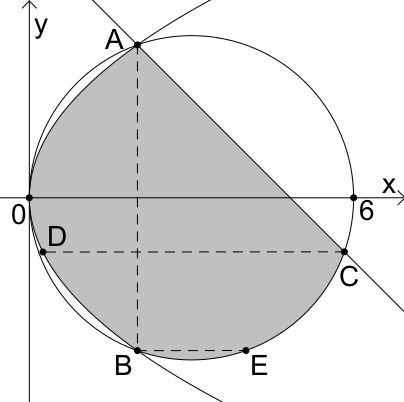
\includegraphics[width=0.4\columnwidth]{images/b1p2-368-fig01}
\end{figure}

It is reasonable to use the first splitting for this problem since the number of subregions is less than that of the other case. But in some problems such a selection may arise difficulty in integration.

Then our regions AODB, and ABEC are respectively:
\begin{align*}
	R_{xy}^{1} &= 
		\{ (x, y): 
		0 \leq x \leq 2,
		\ -2\sqrt{x} < y < 2\sqrt{x} \} 
		= (0,\ 2;
		\ -2\sqrt{x},\ 2\sqrt{x})  \\
	R_{xy}^{2} &= 
		\{ (x, y): 
		2 \leq x \leq 3+2\sqrt{2},
		\ -\sqrt{6x-x^{2}} \leq y \leq -x+2(1+\sqrt{2})\} \\
		& = (2,\ 3+2\sqrt{2};
		\ -\sqrt{6x-x^{2}},\ -x+2(1+\sqrt{2})) \\
	\hAbs{A} & = 
		\hAbs{R_{xy}^{1}}+\hAbs{R_{xy}^{2}} \\
	& = \int_{0}^{2} 
		(2\sqrt{x}-(-2\sqrt{x})) \, \hDif x 
		+\int_{2}^{3+2\sqrt{2}} 
			\!\!\! -x+2(1+\sqrt{2})-(-\sqrt{6x-x^{2}})) \, \hDif x \\
	& = \frac{16}{3} \sqrt{2} 
		+ \frac{7}{2} 
		+ \int_{2}^{3+2\sqrt{2}} 
			\sqrt{6x-x^{2}} \, \hDif x
\end{align*}
Writing $6x-x^{2}=9-(x-3)^{2}$ and setting $x-3=3\sin t$ we have
\begin{align*}
	\int \sqrt{6x-x^{2}} \, \hDif x 
	&= \int 
		\sqrt{9-9 \sin^{2} t} \cdot 3 \cos t \, \hDif t \\
	& = 9 \int 
		\cos^{2} t \, \hDif t 
	= \frac{9}{2} (t+ \frac{\sin 2t}{2}) + c \\
	\alpha = 
		\int_{2}^{3+2\sqrt{2}} 
			\sqrt{6x-x^{2}} \, \hDif x
	&= \frac{9}{2} \arcsin \frac{2 \sqrt{2}}{3} 
		+ \arcsin \frac{1}{3} + \frac{4 \sqrt{2}}{9}\\
	A = \frac{16}{3} \sqrt{2} + \frac{7}{2} + \alpha .
\end{align*}
% ++++++++++++++++++++++++++++++++++++++
\hPage{b1p2/371}
% ++++++++++++++++++++++++++++++++++++++
\begin{thm}
	\footnote{proof of theorem continues from the previous page, 'THEOREM' and 'PROOF' words are not undesirable in my page.}
	\begin{proof}
		will be $-h,\:h$ so that
		\begin{align*}
			A &= \int_{-h}^{h} \! (\alpha x^{2} + \beta x + \gamma)\, \hDif x = (\frac{\alpha}{3}x^{3} + \frac{\beta}{2}x^{2} + \gamma x)_{-h}^{h} \\
			&= \frac{2}{3} \alpha h^{3} + 2 \gamma h = \frac{h}{3} (2 \alpha h^{2} + 6\gamma)
		\end{align*}
		Since,
		\begin{align*}
			y_{0} &= \alpha h^{2} - \beta h + \gamma \\
			4y_{1} &= \qquad\qquad\quad 4\gamma \\
			y_{2} &= \alpha h^{2} + \beta h + \gamma \\
			\cline{1-2}
			y_{0}+4y_{1}+y_{2} &= 2\alpha h^{2} \qquad +6\gamma
		\end{align*}
		we have our result.
		\par Now partitioning $\hPairingParan{a,b}$ regularly for an even number $n$ and applying the above lemma for consecutive pairs of strips and adding the results of each pair, we have
		\begin{align*}
			\frac{h}{3} ((y_{0}+4y_{1}+y_{2})+(y_{2}+4y_{3}+y_{4})+\cdots +(y_{n-2}+4y_{n-1}+y_{n}))
		\end{align*}
		and
		\begin{align*}
			\int_{a}^{b} \! f(x)\, \hDif x = \frac{h}{3}(y_{0}+4y_{1}+2y_{2}+4y_{3}+\cdots +2y_{n-2}+4y_{n-1}+y_{n})
		\end{align*}
		where $h=(b-a)/n$ and $n$ is an even number.
		\par Observe that coefficients of $y_{1}$ are $1$ for $i=0$ and $i=n$; for others, $4$ for odd $i$ and $2$ for even $i$.
	\end{proof}
\end{thm}

\begin{exmp}
	Evaluate the definite integral
	\begin{align*}
		A = \int_{1}^{3}\frac{\hDif x}{x}
	\end{align*}
	approximately (numerically) using the three rules, taking $n=6$.
	\begin{hSolution}
		\footnote{solution of the example continues to the next page. In order not to get errors while compiling, I closed my tags here.}
		We have $h=\frac{3-1}{6}=\frac{1}{3}$ and
		\begin{align*}
			\begin{tabular}{c|cccccccc|}
				$x_{i}$ & $1$ & $\frac{4}{3}$ & $\frac{5}{3}$ & $2$ & $\frac{7}{3}$ & $\frac{8}{3}$ & $3$ \\
				\hline
				$y_{i}$ & $1$ & $\frac{3}{4}$ & $\frac{3}{5}$ & $\frac{1}{2}$ & $\frac{3}{7}$ & $\frac{3}{8}$ & $\frac{1}{3}$
			\end{tabular}
		\end{align*}
	\end{hSolution}
\end{exmp}


% ++++++++++++++++++++++++++++++++++++++
\hPage{b1p2/402}
% ++++++++++++++++++++++++++++++++++++++


% =====================================

\begin{exmp} \footnote{The example's solution starts in the previous page. 
			        Begin tags should be removed.}

	\begin{hSolution}
		\begin{hEnumerateAlpha} 
			\item \footnote{This is the b part, a part is in the previous page. 
					     Begin tag should be removed.}
   			\begin{align*}
					y = 
						(1 + \frac{1}{x})^x 
						\Rightarrow 
						\ln y =\:x\ln&(1 + \frac{1}{x})\\
	  		\ln (\lim_{x\to\infty} y) = 
							         &\lim_{x\to\infty} 
											\left( x\ln(1 +
													\frac
														{1}
														{x}
									      			      )\right) = 
														(\infty,0)\\
				   	       	                = &\lim_{x\to\infty} 
										\frac
											{\ln(1+\frac{1}{x})}
											{1/x} 
														= \lim_{x\to\infty}
																	\frac
																		{\frac
																			{-1/x^2}
																			{1 + 1/x}
																		}
																		{-1/x^2} 
																						= 1 = \ln e\\
		   	 		           \Rightarrow &\lim_{x\to\infty} y = e
			\end{align*}
		\end{hEnumerateAlpha}
	\end{hSolution}

\end{exmp}

% =====================================

\begin{exmp}

	Evaluate $\lim_{x\to 0} (\cos 2x)^{1/x^2}$

	\begin{hSolution}
		\begin{alignat*}{2}
			y = (\cos 2x)^{1/x^2} 
				&\Rightarrow \ln y &&= \frac{1}{x^2}
										\ln \cos 2x\\
	 \ln(\lim_{x\to 0} y) &= \lim_{x\to 0}    &&\frac
								{\ln \cos 2x}
								{x^2} 
										= \left( \frac{0}{0} \right) 
														= \lim_{x\to 0} 
																\frac
																	{\frac
																		{-2 \sin 2x}
																		{\cos 2x}
																	}
																	{2x} \\
				&= -2                     &&\lim_{x\to 0} 
									(\frac
										{\sin 2x}
										{2x} 
									 \frac
										{1}
										{\cos 2x}
									) = -2 = \ln e^{-2}\\
				&\Rightarrow         &&\lim_{x\to 0} y = e^{-2}
		\end{alignat*}
	\end{hSolution}

\end{exmp}

% =====================================

\textbf{Sketching.} The procedure for sketching the curve of 
$y = u(x)^{v(x)}$ is the same as that given for the case $u(x)$ is a constant function. 
One determines first the domain, and makes a table of variation for $u(x)$ and $v(x)$ 
and get the values or limits of $y$ corresponding to the specific values obtained for x in the table.\\

% =====================================

\begin{exmp}

	Sketch the curves of

	\begin{multicols}{2}
		a) $y = f(x) = x^x$
	
		b) $f(x) = (1+x)^{1/x}$
	\end{multicols}

	\begin{hSolution}

		a) $\textrm{D}_f = (0,\infty)$
	

		$y^\prime = x^x(1+\ln x) = 0 \Rightarrow x = 1/e$

	\end{hSolution}

\end{exmp}
%++++++++++++++++
 \hPage{b1p2/417}
%++++++++++++++++++++
    \begin{center}
        \includegraphics{images/b1p2-417-fig01.png}
    \end{center}
    
    We are going to show that $\Theta$ as arc $(angle)$ on the unit
    circle represents the area of the shaded segment of circle bounded by the line segment $(OP),$ $(OP^\prime)$ and the arc $P^\prime AP$, and $\Theta$ as argument in hyperbolic functions represents the area of the shaded region bounded by $(OP),$ $(OP^\prime)$ and the arc of hyperbola $P^\prime AP$.
    
    \begin{hEnumerateAlpha}
        \item $|OP^\prime AP \vert = \frac{2\Theta}{2\Pi} $ $ \Pi r^2 $ $(r = 1) = \Theta$
        \item $|OP^\prime AP \vert = 2 |POH \vert -2|PAH \vert = \operatorname{Ch}\Theta \operatorname{Sh}\Theta - 2 \int_A^P y \,dx$
    \end{hEnumerateAlpha}
    
    $ $\\
    \noindent
    where, having 
    
    \begin{align*}
        2 \int_A^P y \,dx &= 2 \int_0^\Theta \operatorname{Sh}t \,d\operatorname{Ch}t = 2 \int_0^\Theta \operatorname{Sh}t^2 \,dt
        \\
        &= 2 \int_0^\Theta (\operatorname{Ch}2t - 1) \,dt = \frac{1}{2} \operatorname{Sh}2\Theta - \Theta ,
    \end{align*}
    
    \noindent
    we get 
    
    \[
        |OP^\prime AP \vert = \operatorname{Ch}\Theta \operatorname{Sh}\Theta - \frac{1}{2} \operatorname{Sh}2\Theta + \Theta = \Theta
    \]
    
    \section{INVERSE HYPERBOLIC FUNCTIONS.}
    
    Observing from the graphs of hyperbolic functions the all these, except $\operatorname{Ch}x$ and $\operatorname{Sech} x$ are monotone increasing or monotone decreasing on their domain, while\footnote{Since $\operatorname{Ch} x$ ($\operatorname{Sech} x$) is monotone decreasing (increasing) ($-\infty , 0$) also inverse in that interval and the graphs is symmetric of the given one w.r. to x-axis.} $\operatorname{Ch}x$ $\operatorname{Sech} x$
%%%%%%%%%%%%%%%%%%%%%%%%%%%%%%%%%%%%%%%%%%%%
\hPage{b1p2/423} 
%%%%%%%%%%%%%%%%%%%%%%%%%%%%%%%%%%%%%%%%%%%
\footnote{Package used: mdframed for the box without bottom part}
\footnote{Package used: mathbx to get $\rightbarharpoon$ (instead we can use $\Rightarrow$ )}
\footnote{Package used: graphbox to align the images}
\footnote{Set the mdframe option:newmdenv[bottomline=false]\{notbottom\}}

\begin{hEnumerateArabic}
    \item[]
        \begin{hEnumerateAlpha}
            \item \( { ( Ch x + Sh x )}^{- Argch x} = { ( ch x - Sh x )}^{- Argsh (x-2)}  \)
            \item \( Ch 7x + Ch 5x + Ch 3x = Ch 6x + Ch 4x + Ch 2x \)
        \end{hEnumerateAlpha}
\end{hEnumerateArabic}
\section*{ANSWERS TO EVEN NUMBERED EXERCISES}
\begin{hEnumerateArabic}
    \setcounter{enumi}{5}
    \item 24/7, 25/7, 24/25 , 7/25, 7/24, 25/24.
    \setcounter{enumi}{47}
    \item 
        \begin{hEnumerateAlpha}
            \item R, $(2x + 2) Ch(x^2 + 2)$,
            \item R, $-(2x - 2) Sech(x^2 - 2x) Th(x^2 - 2x)$
        \end{hEnumerateAlpha}
    \setcounter{enumi}{51}
    \item 
        \begin{hEnumerateAlpha}
            \begin{multicols}{2}
                \item $-\csc x$,
                \columnbreak
                \item $\csc x$
            \end{multicols}
        \end{hEnumerateAlpha}
    \setcounter{enumi}{53}
    \item
        \begin{hEnumerateAlpha}
            \begin{multicols}{2}
                \item \includegraphics[align=t,scale=0.75]{images/b1p2-423-fig01.png}
                \columnbreak
                \item \includegraphics[align=t,scale=0.75]{images/b1p2-423-fig02.png}
            \end{multicols}
        \end{hEnumerateAlpha}
    \setcounter{enumi}{57}
    \item
        \begin{hEnumerateAlpha}
            \begin{multicols}{2}
                \item \( \ln \sqrt{3}\)  
                \columnbreak
                \item 0
            \end{multicols}
        \end{hEnumerateAlpha}
    \setcounter{enumi}{59}
    \item
        \begin{hEnumerateAlpha}
            \begin{multicols}{2}
                \item 5/4  
                \columnbreak
                \item 0
            \end{multicols}
        \end{hEnumerateAlpha}
\end{hEnumerateArabic}
\section*{A SUMMARY}
\begin{notbottom}
    \begin{hEnumerateArabic}
        \item[6.1]
            \begin{hEnumerateAlpha}{}
                \item[] \(\ln x = \int_{1}^{x} \frac{dt}{t} (x > 0), \ln 1 = 0, \ln e = 1 \)
                \item[] \(\ln ab = \ln a + \ln b, \ln \frac{a}{b} = \ln a - \ln b\)
                \item[] \(\log_b x = \log_a x \cdot \log_b a\) (change of base)
                \item[] \(\frac{d}{dx} a^{u(x)} = a^u \frac{du}{dx} \ln u, \frac{d}{dx} \log_a u(x) = \frac{1}{u} \frac{du}{dx} \log e  \)
                \item[] \(\frac{d}{dx} u(x)^{v(x)} = u^v \big(\frac{dv}{dx} \ln u +  \frac{v}{u} \frac{du}{dx} \big)  \)
                \item[] \( y = uv \ldots w \rightbarharpoon \frac{y^\prime}{y} = \frac{u^\prime}{u} + \frac{v^\prime}{v} + \ldots + \frac{w^\prime}{w} \text{(logarithmic derivative)} \)
            \end{hEnumerateAlpha}
    \end{hEnumerateArabic}
\end{notbottom}
% ++++++++++++++++++++++++++++++++++++++
\hPage{b1p2/435}
% ++++++++++++++++++++++++++++++++++++++
\[
	+(\frac{C_1x + D_1}{x^2+px+q} + ... + \frac{C_{\lambda}x + D_\lambda}{(x^2+px+q)^\lambda})+(\frac{E_1x+F_1}{x^2+rx+s}+...+\frac{E_\mu x+ F_\mu}{(x^2+rx+s)^\mu})+...
\]
of finite number of partial fractions with $A_\alpha \neq 0,  B_\beta \neq 0, ... ,C_\lambda x + D_\lambda \neq 0,\hspace{3mm}  E_\mu x + F_\mu \neq 0.$

\begin{proof}
	See Appendix at the end of the book.
\end{proof}

By this theorem, in the decomposition, to a real root of multiplicity $\nu$ correspond $\nu$ partial fractions (some of which may be zero), and to a pair of conjugate imaginary roots of common multiplicity $\nu$ correspond $\nu$ partial fractions (some of which may be zero).

For instance
\begin{enumerate}

	\item[1.]
 	$\frac{x^6-2x+5}{(x-1)x^3(x^2+1)^2} = \frac{A}{x-1} + (\frac{B_1}{x}+\frac{B_2}{x^2}+\frac{B_3}{x^3})+(\frac{C_1x+D_1}{x^2+1}+\frac{C_2x+D_2}{(x^2+1)^2})$

	\item[2.] 
	$\frac{3}{(x-1)^2}= \frac{A}{(x-1)^2} \quad (\Rightarrow A=3, why?)$
	
	\item [3.] 
	$\frac{2x^2-7}{(x^2-x+1)^3}=\frac{A_1x+B_1}{x^2-x+1}+\frac{A_2x+B_2}{(x^2-x+1)^2}+\frac{A_3x+B_3}{(x^2-x+1)^3}$

\end{enumerate}

We remark that as in (2) above, the decomposition of a partial fraction consists of a single term which is the given fraction.

\begin{exmp}
	Decompose the proper rational function
	\[
		\frac{x^2+15}{(x-3)(x^2-2x-3)}
	\]
	into partial fractions.
\end{exmp}

\textbf{Solution}. Since $x^2-2x-3$ has positive discriminant, it can be factored:  $x^2-2x-3 = (x-3)(x+1)$.

Thus the given fraction is to be written as

%%%%%%%%%%%%%%%%%%%%
\hPage{b1p2/438}
 reducible to integrals of the form
    
    $$A = \int_{}^{} {{1}\over{{(x-a)}^n}} dx, B = \int_{}^{} {{ax+b}\over{({x^2+px+q})^n}} dx$$
    
    of which the (A) is easily integrable by the substitu-\\
    tion $u=x-a$, $du=dx$\\.
    \paragraph{} The second one (B) is reducible to (A) if \\
    $$ax+b=D(x^2+px+q)=2x+p;$$
    otherwise, writing $ax+b$ as
    $$ax+b={{a}\over{2}}(2x+p) + (b- {{ap}\over{2}})$$
    we have
    $$B={{a}\over{2}}\int_{}^{} {{2x+p}\over{(x^2+px+q)^n}}dx+(b-{{ap}\over{2}})\int_{}^{}{1\over{(x^2+px+q)^n}}dx$$
    $$={{{a}\over{2}}\int_{}^{}{{du}\over{u^n}}+c\int_{}^{}{1\over{(x^2+px+q)^n}}dx}$$
    
    where $u=x^2+px+q$ in the first integral. In the second integ-\\
    ral, writing
    $$x^2+px+q=(x+{{p}\over{2}})^2+(x-{{p}\over{2}})^2.$$
    $$={{(x+{{p}\over{2}})^2}+{({{\sqrt{-(p^2-4q)}}\over{2}})^2}}, (\Delta=p^2-4q<0)$$
    
    and setting
    
    $$x+{{p}\over{2}}={{{\sqrt{-\Delta}}\over{2}}u}, dx={{{\sqrt{-\Delta}}\over{2}}du}$$
    
    we have
    
    $$x^2+px+q={({{{\sqrt{-\Delta}}\over{2}}u})^2+({{{\sqrt{-\Delta}}\over{2}}})^2}={{{-\Delta}\over{4}}(u^2+1)}$$
    
    and the integral reduces to
    
    $$k\int_{}{}{{1}\over{(u^2+1)^n}}du$$
    
    which, omitting k and replacing u by x, becomes
    
    $$ {I_{n}} = {\int_{}{}{{dx}\over{(x^2+1)^n}}}$$
    
%%%%%%%%%%%%%%%%%%%%%%%%%%%55 
\hPage{b1p2/444}
%%%%%%%%%%%%%%%%%%%%%%%%%%%
\begin{hEnumerateAlpha}
\setcounter{enumi}{4}
\item $\begin{aligned}\frac{Ax+B}{x^{2}+x+1} + \frac{Cx+D}{x^{2}-x+1}\end{aligned}$
\item $\begin{aligned}\sum_{i=1}^4 \frac{A_{i}}{(x-1)^{i}} + \sum_{i=1}^4 \frac{B_{i}}{(x+1)^{i}} + \sum_{i=1}^3 \frac{C_{i}}{(x-\sqrt{2})^{i}} + \sum_{i=1}^3 \frac{D_{i}}{(x+\sqrt{2})^{i}}\end{aligned}$
\item $\begin{aligned}\frac{A}{x} + \frac{B}{x^{2}} + \frac{C}{x^{3}} + \frac{D}{x+1} + \frac{E}{(x+1)^{2}} + \frac{F}{x-2}\end{aligned}$
\end{hEnumerateAlpha}

\begin{hEnumerateArabic}

\setcounter{enumi}{3}
\item $\begin{aligned} I_{n} = \frac{x^{n-1}}{n-1} - I_{n-2}\end{aligned}$

\stepcounter{enumi}
\item $\begin{aligned}-\frac{2}{x} + \frac{1}{x^{2}} + \frac{1}{x^{3}} + \frac{2x-1}{x^{2}+1} + \frac{x-1}{(x^{2}+1)^{2}} + C\end{aligned}$

\stepcounter{enumi}
\item
\begin{hEnumerateAlpha}
\item $\begin{aligned}\frac{1}{3}\ln\frac{(x+1)^{2}(x-2)}{(x-1)(x+2)^{2}} + C\end{aligned}$
\item $\begin{aligned}\frac{1}{6}\ln\frac{x-1}{x+1} + \frac{\sqrt{2}}{3}\arctan\frac{x}{\sqrt{2}} + C\end{aligned}$
\item $\begin{aligned}\frac{3}{4}\ln\frac{x^{2}+1}{(x-1)^{2}} - \arctan{x} - \frac{3x-4}{2(x-1)^2} + C\end{aligned}$
\end{hEnumerateAlpha}

\stepcounter{enumi}
\item $\begin{aligned}-\frac{3x^{3}+2x^{2}+2x+1}{2x^{2}(x^{2}+1)} + \ln\frac{x^{2}+1}{x^{2}} - \frac{3}{2}\arctan{x} + C\end{aligned}$

\stepcounter{enumi}
\item
\begin{hEnumerateAlpha}
\item $\begin{aligned}\ln\frac{x}{x-1} - \frac{1}{6}\ln{(x^{2}+1)} - \frac{1}{3}\arctan{x} - \frac{x+1}{x^{2}+1} + C\end{aligned}$
\item $\begin{aligned}\frac{1}{\sqrt{11}}\arctan\frac{4x+1}{\sqrt{11}} + C\end{aligned}$
\end{hEnumerateAlpha}

\stepcounter{enumi}
\item
\begin{hEnumerateAlpha}
\item $\begin{aligned}\ln{(x-2)^{2}}|x+2|^{3} + 6\end{aligned}$
\item $\begin{aligned}\frac{5}{9}\ln{|x-1|} + \frac{4}{9}\ln{|x+2|} - \frac{1}{3(x-1)} + C\end{aligned}$
\item $\begin{aligned}\ln{(x-1)^{4}} + \frac{1}{3}\ln{|x+1|} + \frac{5}{3}(x-2) + C\end{aligned}$
\item $\begin{aligned}\ln{|x|} - \frac{3}{x+1} + C\end{aligned}$
\end{hEnumerateAlpha}

\stepcounter{enumi}
\item
\begin{hEnumerateAlpha}
\item $\begin{aligned}\frac{1}{2}\ln|2x+1| - 3\arctan{x} + C\end{aligned}$
\item $\begin{aligned}\frac{1}{12}\ln{\left|\frac{2x-3}{2x+3}\right|} + C\end{aligned}$
\end{hEnumerateAlpha}

\stepcounter{enumi}
\item
\begin{hEnumerateAlpha}
\item $\begin{aligned}\ln\frac{9}{8}\end{aligned}$
\item $\begin{aligned}\frac{3}{28} + \ln{16}\end{aligned}$
\end{hEnumerateAlpha}

\stepcounter{enumi}
\item $\begin{aligned}\ln\frac{9}{2}\end{aligned}$

\end{hEnumerateArabic}
%%%%%%%%%%%%%%+++++++
\hPage{b1p2/447}
%+++++++++++++++++++++++
\begin{exmp}


Evaluate B = $\int \! \frac{1}{2Sh\theta - 3Ch\theta +1} \, \hDif \theta $\\
\begin{hSolution}
Th$\frac{\theta}{2}=t\quad\Longrightarrow
\quad\theta =2Argtht\quad\Longrightarrow
\quad\hDif \theta =\frac{2\hDif t}{1-t^{2}}$ , and\\
\begin{align*}
Sh\theta=\frac{2t}{1-t^{2}}\quad , \quad Ch\theta=\frac{1+t^{2}}{1-t^{2}}\\
\end{align*}
\begin{align*}
B
&=\int \! \frac{1}{\frac{-4t}{1-t^{2}}-3\frac{1+t^{2}}{1-t^{2}}+1}\frac{2\hDif t}{1-t^{2}}=-2 \int \! \frac{\hDif t}{4t^{2}-4t+2}\\
&=\int \! \frac{\hDif (2t)}{(2t)^{2}-2(2t)+2}=-\int \! \frac{\hDif u}{u^{2}-2u+2} \qquad (u=2t)\\
&=-\int \! \frac{\hDif (u-1)}{(u-1)^{2}+1}=-arctan(u-1)+C\\
&=-arctan(2t-1)+C=-arctan(2Th\frac{\theta}{2}-1)+C.\\
\end{align*}
\end{hSolution}
\end{exmp}
\par The half-angle (half-argument) substitutions works always for the rational integrands in trigonometric (or hyperbolic) functions.\\
\par In some cases as the following ones the use of these substitutions not necessary:\\
\par \underline{Integrals reducible to $\int \! \hDif  u /u$}:\\
\begin{multicols}{2}
\begin{enumerate}
\item
$
\!
\begin{aligned}[t]
 a)&\int \! tan\theta \hDif \theta\\
&\int \! tan\theta \hDif \theta =\int \! \frac{sin\theta}{cos\theta}\hDif \theta\\
=& \int \! \frac{-\hDif cos\theta}{cos\theta}=-ln\hAbs{cos\theta}+c\\
\end{aligned}
$ 
\begin{align*}
b)&\int \! cot\theta \hDif \theta = \int \! \frac{\hDif sin\theta}{sin\theta}\\
=&ln\hAbs{sin\theta}+c\\
\end{align*}
\begin{align*}
a')&\int \! Th\theta \hDif \theta\\
&\int \! Th\theta \hDif \theta = \int \! \frac{Sh\theta}{Ch\theta} \hDif \theta\\
=&\int \! \frac{\hDif ch\theta}{ch\theta}=ln\quad ch\theta+c.\\
\end{align*}
\begin{align*}
b')&\int \! Coth\theta \hDif \theta = \int \! \frac{\hDif Sh\theta}{Sh\theta}\\
=&ln\hAbs{Sh\theta}+c.\\
\end{align*}
\end{enumerate}
\end{multicols}
%+++++++++++++++++++++++++++++
\hPage{b1p2/460\footnote{Following functions were declared as math operators above to keep function style and syntax: $\Sh{x}$, $\Ch{x}$, $\Sech{x}$, $\Th{x}$}}
%+++++++++++++++++++++++++++
We transform A${x}^2$ + Bx + C as follows:
\begin{align*}
    A{x}^2 + Bx + C &= A\left({x}^2 + \frac{B}{A}x + \frac{C}{A}\right) \\
    &= A\left({(x + \frac{B}{2A})}^2 - \frac{{B}^2}{4{A}^2} + \frac{C}{A}\right) \\
    &= A\left({(x + \frac{B}{2A})}^2 - \frac{{B}^2 - 4AC}{4{A}^2}\right)
\end{align*}
\\
Setting
\begin{align*}
    x + \frac{B}{2A} &= u
\end{align*}

we have
\begin{align*}
    A{x}^2 + BX + C &=
    A\left({u}^2 - \frac{\Delta}{4{A}^2}\right) \cdot (\Delta = {B}^2 - 4AC)
\end{align*}

\par If A $>$ 0, then
\begin{align*}
    A{x^2} + Bx + C \text{ involves }
    \left(
    \begin{array}{lll}
         {u}^2 - {a}^2 & when & \Delta > 0 \\
         {u}^2 + {a}^2 & when & \Delta < 0
    \end{array}
    \right.,
\end{align*}
and if A $<$ 0, it involves ${a}^2 - {u}^2$.

\begin{table}[h]
    \centering
    \caption{}
    \begin{tabular}{cccc}
            Integrand involved &
            Substitution &
            New integrand involves &
            ${du}$
            \\ \hline%------------
            ${u}^2 + {a}^2$
            &
            $
            \left(
                \begin{array}{c}
                    u = a \tan{t}\\
                       or\\
                    u = a \Sh{t}
                \end{array}
            \right.
            $
            &
            $
            \left( 
            \begin{array}{c}
                     {a}^2 \sec^2{t}\\
                        or\\
                     {a}^2 \Ch^2{t}
                \end{array}
            \right.
            $
            &
            $
            \left(
                \begin{array}{c}
                    {a} \sec^2{t} {dt} \\
                        or \\
                    {a} \Ch{t} {dt}
                \end{array}
            \right.
            $
            \\[8mm]%------------
            ${u}^2 - {a}^2$
            &
            $
            \left(
                \begin{array}{c}
                    u = a \sec{t} \\
                        or\\
                    u = a \Ch{t}
                \end{array}
            \right.
            $
            &
            $
            \left(
                \begin{array}{c}
                    {a}^2 \tan^2{t} \\
                        or \\
                    {a}^2 \Sh^2{t}
                 \end{array}
            \right.
            $
            &
            $
            \left(
                \begin{array}{c}
                    {a} \sec{t} \tan{t} {dt} \\
                        or \\
                    {a} \Sh{t} {dt}
                \end{array}
            \right.
            $
            \\[8mm]%-=-=-=-=-=-=-=-=-=
            ${a}^2 - {u}^2$
            &
            $
            \left(
                \begin{array}{c}
                    {u} = {a} \sin{t}\text{\footnotemark} \\
                        or \\
                    {u} = {a} \Th{t}
                \end{array}
            \right.
            $
            &
            $
            \left(
                \begin{array}{c}
                    {a}^2 \cos^2{t} \\
                        or \\
                    {a}^2 \Sech^2{t}
                \end{array}
            \right.
            $
            &
            $
            \left(
                \begin{array}{c}
                    {a} \cos{t} {dt} \\
                        or \\
                    {a} \Sech^2{t} {dt}
                \end{array}
            \right.
            $
    \end{tabular}
\end{table}
\footnotetext{The substitution ${u}={a}$ cost works also, but ${u}={a} \sin{t}$ is preferred}
% ++++++++++++++++++++++++++++++++++++++
\hPage{b1p2/469}
% ++++++++++++++++++++++++++++++++++++++
	
	a) $\int x \sqrt{\frac{1+x}{1-x}}dx$ \quad
    	b) $\int^2_0 {\frac{\sqrt{x+1}-1}{\sqrt{x+1}+1}}dx$	
	
	\begin{enumerate}
		

    	\item[81.]
    	Evaluate $\int^b_a \frac{dx} {\sqrt{(x-a)(b-x)}}$

    	\item[82.]
    	If R(x, $\sqrt{ax^2 + bx + c}$ is a rational function of its arguments, show that it becomes a rational function of t upon the substitution: \\
    	a) $ t = \sqrt{a}x+\sqrt{ax^2 + bx + c}$ when $a > 0,$\\
    	b) $ t = \sqrt{(-a).\frac{x - x_1}{x_2 - x}}$ when $a < 0$, where $x_1, x_2$ are the (real) roots of $ax^2+bx+c=0 (x_1 < x_2)$

    	\item[83.]
    	Apply the substitution given in Exercise 82 to transform\\
   	a)$\int\frac{3-\sqrt{4x^2+x-1}}{x+\sqrt{4x^2+x-1}}dx$
    	b)$\int\frac{\sqrt{x - x^2}}{1 + \sqrt{x - x^2}}dx$ \\
    	into ones with integrand as rational function of t.

    	\item[84.]
    	Evaluate $\int \frac{1-\sqrt[3]{x}}{\sqrt{x}}dx$

    	\item[85.]
    	Show that $\int^\pi_0 \frac{x \sin x}{1+\cos ^2x}dx = \frac{\pi^2}{4}$

    	\item[86.]
    	Find the area of the region bounded by the x-axis, the curve $y=xe^{-x}$ and the vertical line through the maximum point.

    	\item[87.]
    	Evaluate $\int x e^x \cos x dx$

    	\item[88.]
    	Find the area between the two curves:\\
    	a)$y=\ln x, y = \ln \frac{1}{x}, 1 < x < e $ \\
    	b)$y=\sin ^2x,y = \sec x, \frac{2\pi}{4} < x < \frac{5\pi}{4}$

    	\item[89.]
    	Given $I_n = \int \cos (n \arctan x)dx$, show that $I_{n+2} + 2I_n + I_{n-2} = \frac{4}{n} \sin (n \arctan x)+c$ 

    	\item[90.]
    	Determine the convergence or divergence, and find the value

	\end{enumerate}
% ++++++++++++++++++++++++++++++++++++++
\hPage{b1p2/482}
% ++++++++++++++++++++++++++++++++++++++

\subsection{Volume of a Solid of Revolution}:
\label{subsec:VolumeofaSolidofRevolution}
\\
A \hDefined{solid of revolution} is the solid generated by revolving a plane region about a (straight) line. This line is called the symmetry axis of the solid. The boundary of a surface of revolution is certainly a surface of revolution.
\\
Consider first a region under the curve of a continuous positive function \(y=f(x)\) bounded by the lines \(x=a, x=b.\)
\\
When this region is revolved about the x-axis (or the y-axis), it generates a solid of revolution whose volume is denoted by \(V_{ox}\) (or \(V_{oy}\)).
\begin{figure}[htb]
	\centering
    \includegraphics[width=.4\textwidth]{images/b1p2-482-fig01}
\end{figure}
\\
For this region, for convenience \(V_{ox}\) will be evaluated by what we call \hDefined{disc method}, while \(V_{oy}\) by \hDefined{shell method} as explained below.
\\
Consider an element of area as a vertical strip in the region R. When R is rotated about x-axis (y-axis) the strip generates an element of volume in the form of a \hDefined{disc} (a \hDefined{shell})
\begin{figure}[htb]
	\begin{minipage}{0.45\textwidth}
		\centering
    	\includegraphics[width=\textwidth]{images/b1p2-482-fig02}
		\caption{Disc of radius y and thickness dx}
	\end{minipage}
	\begin{minipage}{0.45\textwidth}
		\centering
    	\includegraphics[width=\textwidth]{images/b1p2-482-fig03}
		\caption{Shell of inner radius x, thickness dx and height y.}
	\end{minipage}
\end{figure}

%%%%%%%%%%%%%%%%%%%%
\hPage{b1p2-497}
%%%%%%%%%%%%%%%%%%%%%%
	\paragraph{}$M_{ox} = 
	\begin{cases}	\int_{a}^{b} \  f(x) \ \delta{x} \ \sqrt{1 + f^{'^{2}}(x)}\hDif {x} \\ \int_{c}^{d} \  y \ \delta{y} \ \sqrt{1 + g^{'^{2}}(y)}\hDif {y}, \\ \end{cases}$ \\ 
	\paragraph{}$M_{oy} = \begin{cases} \int_{a}^{b} \ x \ \delta{x} \ \sqrt{1 + f^{'^{2}}(x)}\hDif {x} \\ \int_{c}^{d} \ g(y) \ \delta{y} \ \sqrt{1 + g^{'^{2}}(y)}\hDif {y}. \\ 
	\end{cases}$
	\paragraph{}We define the \textit{center of mass (center of gravity)} of the arc with mass as the point G($\overline{x}$, $\overline{y}$) such that the moments m$\overline{y}$, m$\overline{x}$ of the particle G(m) are the same as the moments $M_{ox}$, $M_{oy}$ of the arc where m is the total mass of the arc:
	\begin{align*}
		m \overline{x} &= M_{oy} \ ,  &m\overline{y}= M_{ox}
	\end{align*}
	These defined equalities give
	\begin{align*}
		  \overline{x} &= \frac{M_{oy}}{m}  \text{,}   &\overline{y} = \frac{M_{ox}}{m}
	\end{align*}
	as coordinates of the center of mass G. 
	\paragraph{}$\underline{Example}$. Find the center of mass of a wire bent in the shape of semi circle $x^{2}$ + $y^{2}$ = $a^{2}$ if the density is $\delta{}$ = 2y. \paragraph{}$\underline{Solution}$. Since the arc and the density function are symmetric with respect to y-axis, it follows that G lies on y, axis, and $\overline{x}$ = 0.
	\paragraph{}To find $\overline{y}$, we evaluate first the total mass m of the wire:\\
	\begin{minipage}{0.55\textwidth}
	\begin{align*}
	    m = 2\int_{0}^{a} 2y\sqrt{1 + \frac{y^2}{x^2}} \ \hDif{y} = 4a^2 
	\end{align*}
	Then
	\end{minipage}
	\begin{minipage}{0.45\textwidth}
	\includegraphics[width=\textwidth]{images/b1p2-497-fig01}
	\end{minipage}
	
%++++++++++++++++++++++++++++++++++
    \hPage{b1p2/504}
%+++++++++++++++++++++++++++++++
    \begin{hEnumerateAlpha}
        \item to the top of the tank, 
        \item to a level k ft above the top of the tank.
    \end{hEnumerateAlpha}
    
    \begin{hEnumerateArabic}
        \setcounter{enumi}{42}
    
        \item A trough 20 ft long has a cross section in the shape of an isoceles trapezoid with a lower base 4 ft long, an upper base 10 ft long and an altitude of 4 ft. How much work is done in filling the trough with water if the bottom of the trough is located 20 ft above the pump and the water is pumped in through a valve in the bottom of the trough?
     
        \item A force of 20 kg is required to compress a spring 20 cm long to 19 cm. What is the work done in stretching the spring from a length of 24 cm to 30 cm?
        
        \item A vertical cylindrical tank 6 dm in diameter and 10 dm height is half full of water. Find the amount of work done in pumping all the water to the top of the tank.
        
        \item According to NEWTON's law of universal gravitation two objects of weights $w_{1}$, $w_{2} $ kg are attracted to each other by a force of
              $$k \frac{w_{1}w_{2}}{x^2}  kg,$$

        \noindent where x is the distance between the objects and k is a
        constant. Find the work done in separating the objects from a distance of "a meters" to a distance of "b meters" apart.
        
        \item Find the amount of work done in stretching a spring from its natural length of 8 cm to triple that length if a force of 15 kg is needed to triple it natural length.
        
        \item Find moments of the following arc with respect to x- and y- axes, and find also the centroid of the arc if $\delta$ = 1. 
    
    \end{hEnumerateArabic}
% ++++++++++++++++++++++++++++++++++++++
\hPage{b1p2/506}
% ++++++++++++++++++++++++++++++++++++++

	\begin{hEnumerateAlpha}
		\item $3(2, 2)$, $4(2, -2)$, $5(-2, 2)$, $2(-2, -2)$

		\item $6(0, 0)$, $6(8, 0)$, $6(8, 8)$, $3(4, 4)$

		\item $2(1, 3)$, $7(4, 2)$, $6(3, -3)$, $8(-4, 2)$, $5(-3, -4)$.
		
 
	\end{hEnumerateAlpha}	
    
   	 \begin{hEnumerateArabic}
 		 \setcounter{enumi}{58}
  		 \item Use PAPPUS' Theorem to  find the centroid of the region of a semicircle 
         	 of radius a.
         	 \item Use PAPPUS' Theorem to find the volume of the torus generated by 
        	 revolving the area of a circle of radius a, about an axis b($>$a) units 
         	 from the center of the circle. \\
	\end{hEnumerateArabic}
    
    	 ANSWERS TO EVEN NUMBERED EXERCISES
    	\begin{hEnumerateArabic}
    		\setcounter{enumi}{35}
    		\item \( \frac{500}{3} \) $\pi$ ($12,25$ + $\sqrt[]{35}$ + 100)
    		\setcounter{enumi}{37}
   			\item 1000 g gr-cm.  
    		\setcounter{enumi}{39}
   			\item 60 kg-cm.
    		\setcounter{enumi}{41}
                \item
    			\begin{enumerate}[label=\alph*)]
				\item $11$$\pi$$\delta$ $r^2$$h^2$ $/ 492$   
        			\item $\pi$$\delta$$r^2$$h(11h/492 + 7k/24)$
   			\end{enumerate}	
    		\setcounter{enumi}{43}
   		\item 840 kg-cm.
    		\setcounter{enumi}{45}
    		\item $kw_1w_2(1/a -1/b)$ kg-m
           	\setcounter{enumi}{47}
           	\item
			 \begin{enumerate}[label=\alph*)]
				\item $M_{ox}$ = $-8 \sqrt[]{2}$ , $M_{oy}$ = $8 \sqrt[]{2}$ , $G(2, -2)$
       			 	\item $M_{0x}$ = $12\pi$ , $M_{0y}$ = $8\pi$ , $G(2, 3)$.
   			 \end{enumerate}	
    		\setcounter{enumi}{49}
                \item
    			\begin{enumerate}[label=\alph*)]
				\item $(1/2, -3/2)$
        			\item $(10, 192/205)$
    			\end{enumerate}
    		\setcounter{enumi}{51}
                \item
    			\begin{enumerate}[label=\alph*)]
				\item $459/20$, $27/4$, $(3/2, 51/10)$
        			\item $243/10$, $27/4$, $(3/2, 27/6)$
    			\end{enumerate}
                \setcounter{enumi}{53}
                \item
            		\begin{enumerate}[label=\alph*)]
				\item $M_{ox} = M_{oy} = 3/20$, $G(9/20, 9/20)$
       			        \item $M_{ox} = 1/4$ , $M_{oy} = (\pi/2 \sqrt[]{2})-1$ , $G(1/4(\sqrt[]{2}-1), (\pi-2 \sqrt[]{2})/2 \sqrt[]{2}( 											\sqrt[]{2}-1)$
    			\end{enumerate}	
               \setcounter{enumi}{55}
               \item
            		\begin{enumerate}[label=\alph*)]
				\item $(12/5 , 3/4)$
                        	\item $(8/5 , 16/7)$
    			\end{enumerate}
               \setcounter{enumi}{57}
               \item 
            		\begin{enumerate}[label=\alph*)]
				\item $(0 , 2/7)$
                  	        \item $(4 , 4)$
                   	        \item $(1/28 , -1/14)$
    			\end{enumerate}
              \setcounter{enumi}{59}
              \item $2\pi^2a^2b$. 
    \end{hEnumerateArabic}

\end{document}  

